\documentclass[twoside,final]{hcmut-report}

\usepackage[utf8]{inputenc}
\usepackage[T5]{fontenc}
\usepackage[protrusion=false]{microtype}

\usepackage{graphicx, caption}
\usepackage{amsmath}
\usepackage{xcolor}
\usepackage{listings}
\usepackage{multirow,multicol}
\usepackage{enumitem}
\usepackage{hyperref}
\usepackage{float}
\usepackage{booktabs}
\usepackage{longtable}
\usepackage{array}
\usepackage{tabularx}
\usepackage{makecell}
\usepackage{subcaption}
\usepackage{tikz}
\usepackage{pgfplots}
\usepackage{tcolorbox}
\usepackage{lastpage}
\usepackage{natbib}

\definecolor{keywordcolor}{rgb}{0.13,0.13,1} % Blue keywords
\definecolor{stringcolor}{rgb}{0.7,0.13,0.13} % Dark red strings
\definecolor{commentcolor}{rgb}{0.25,0.5,0.35} % Green comments
\definecolor{backgroundcolor}{rgb}{0.97,0.97,0.97} % Light background
\definecolor{numbercolor}{rgb}{0.85,0.65,0.13} % Numbers
\definecolor{darkgreen}{RGB}{0,120,0}

\lstdefinelanguage{Python}{
  morekeywords={
    and, as, assert, async, await, break, class, continue, def, del, elif, else, except,
    False, finally, for, from, global, if, import, in, is, lambda, None, nonlocal, not, 
    or, pass, raise, return, True, try, while, with, yield
  },
  keywordstyle=\color{keywordcolor}\bfseries,
  morekeywords=[2]{bool, bytes, bytearray, complex, dict, float, frozenset, int, list, object, set, str, tuple},
  keywordstyle=[2]\color{blue}\bfseries,
  identifierstyle=\color{black},
  sensitive=true,
  comment=[l]{\#},
  morecomment=[s]{'''}{'''}, 
  morecomment=[s]{"""}{"""},
  commentstyle=\color{commentcolor}\ttfamily,
  stringstyle=\color{stringcolor}\ttfamily,
  morestring=[b]',
  morestring=[b]",
  % Highlight numbers
  literate=
    *{0}{{{\color{numbercolor}0}}}1
    {1}{{{\color{numbercolor}1}}}1
    {2}{{{\color{numbercolor}2}}}1
    {3}{{{\color{numbercolor}3}}}1
    {4}{{{\color{numbercolor}4}}}1
    {5}{{{\color{numbercolor}5}}}1
    {6}{{{\color{numbercolor}6}}}1
    {7}{{{\color{numbercolor}7}}}1
    {8}{{{\color{numbercolor}8}}}1
    {9}{{{\color{numbercolor}9}}}1
    {.0}{{{\color{numbercolor}.0}}}2
    {.1}{{{\color{numbercolor}.1}}}2
    {.2}{{{\color{numbercolor}.2}}}2
    {.3}{{{\color{numbercolor}.3}}}2
    {.4}{{{\color{numbercolor}.4}}}2
    {.5}{{{\color{numbercolor}.5}}}2
    {.6}{{{\color{numbercolor}.6}}}2
    {.7}{{{\color{numbercolor}.7}}}2
    {.8}{{{\color{numbercolor}.8}}}2
    {.9}{{{\color{numbercolor}.9}}}2
    {e+}{{{\color{numbercolor}e+}}}2
    {e-}{{{\color{numbercolor}e-}}}2
    {\#\#NUMSTART\#\#}{}{0}
    {\#\#NUMEND\#\#}{}{0},
}
\lstset{
  language=Python,
  backgroundcolor=\color{backgroundcolor},
  basicstyle=\ttfamily\footnotesize,
  numbers=left,
  numberstyle=\tiny\color{gray},
  stepnumber=1,
  numbersep=10pt,
  tabsize=2,
  showspaces=false,
  showstringspaces=false,
  breaklines=true,
  breakatwhitespace=true,
  frame=single,
}

\lstdefinelanguage{TypeScript}{
  keywords={abstract, as, boolean, break, case, catch, class, continue, const, constructor, debugger, declare, default, delete, do, else, enum, export, extends, false, finally, for, from, function, get, if, implements, import, in, infer, instanceof, interface, is, keyof, let, module, namespace, never, new, null, number, object, of, package, private, protected, public, readonly, require, global, return, set, static, string, super, switch, symbol, this, throw, true, try, type, typeof, undefined, unique, unknown, var, void, while, with, yield, async, await},
  keywordstyle=\color{keywordcolor}\bfseries,
  ndkeywords={string, number, boolean, Promise, any, void},
  ndkeywordstyle=\color{blue}\bfseries,
  identifierstyle=\color{black},
  sensitive=true,
  comment=[l]{//},
  morecomment=[s]{/*}{*/},
  commentstyle=\color{commentcolor}\ttfamily,
  stringstyle=\color{stringcolor}\ttfamily,
  morestring=[b]',
  morestring=[b]",
}

\lstset{
  language=TypeScript,
  backgroundcolor=\color{backgroundcolor},
  basicstyle=\ttfamily\footnotesize,
  numbers=left,
  numberstyle=\tiny\color{gray},
  stepnumber=1,
  numbersep=10pt,
  tabsize=2,
  showspaces=false,
  showstringspaces=false,
  breaklines=true,
  breakatwhitespace=true,
  frame=single,
}
\lstdefinelanguage{EnvCustom}{
  keywords={VITE_APP_API_URL, DATABASE_URL, DB_HOST, DB_USER, DB_PASSWORD, DB_PORT, DB_NAME, JWT_SECRET},
  keywordstyle=\color{blue}\bfseries,
  sensitive=true,
  comment=[l]{\#},
  commentstyle=\color{gray}\ttfamily,
  morestring=[b]',
  morestring=[b]",
  stringstyle=\color{red}\ttfamily,
  identifierstyle=\color{black}
}

\lstdefinelanguage{JavaScriptCustom}{
  keywords={
    break, case, catch, class, const, continue, debugger, default, delete, do, else, export,
    extends, finally, for, function, if, import, in, instanceof, let, new, return, super, 
    switch, this, throw, try, typeof, var, void, while, with, yield, await, async,
    mysql, dotenv, process, config, createPool, getConnection, release
  },
  keywordstyle=\color{blue}\bfseries,
  ndkeywords={true, false, null, undefined, NaN, Infinity},
  ndkeywordstyle=\color{teal}\bfseries,
  identifierstyle=\color{black},
  sensitive=true,
  comment=[l]{//},
  morecomment=[s]{/*}{*/},
  commentstyle=\color{gray}\ttfamily,
  stringstyle=\color{red}\ttfamily,
  morestring=[b]',
  morestring=[b]"
}


\lstdefinelanguage{SQL}
{
  keywords={SELECT, FROM, WHERE, GROUP BY, HAVING, ORDER, BY, CREATE, PROCEDURE, FUNCTION, TRIGGER, BEGIN, END, DECLARE, IF, ELSE, RETURN, SET, INSERT, UPDATE, DELETE, INTO, VALUES, SIGNAL, JOIN, ON, AND, IN, GROUP, AS, RETURNS, DETERMINISTIC, COUNT, IFNULL, SQL, DATA, READS, THEN, AFTER, FOR, EACH, ROW, OLD, NEW, ROUND, CONSTRAINT, FOREIGN, KEY, REFERENCES, PRIMARY, CHECK, TABLE, DEFAULT, DESC, UNION, ALL, OVER, WHILE, DO, LEAVE, EXISTS, BEFORE, OR, IDENTIFIED, GRANT, TO, LEFT, RIGHT},
  keywordstyle=\color{blue}\bfseries,
  morekeywords=[2]{INT, CHAR, VARCHAR, BOOLEAN, DATE, DECIMAL, ENUM, TIME, CASCADE, NULL, NOT, USER, PRIVILEGES, TRUE},
  keywordstyle=[2]\color{red}\bfseries,
  comment=[l]{--},
  commentstyle=\color{gray}\ttfamily,
  morestring=[b]',
  stringstyle=\color{teal},
  basicstyle=\ttfamily\footnotesize,
  showstringspaces=false,
  breaklines=true
}

\lstset
{
  language=SQL,
  frame=single,
  breaklines=true,
  columns=flexible,
  keepspaces=true,
  numbers=left,
  numberstyle=\tiny\color{gray},
  backgroundcolor=\color{white}
}
\newcommand{\sql}[1]
{
  \begin{lstlisting}[language=sql]
    #1
  \end{lstlisting}
}
\newcommand{\python}[1]
{
  \begin{lstlisting}[language=python]
    #1
  \end{lstlisting}
}

\newcommand{\result}[1]{\fcolorbox{red}{white}{#1}}

\AtBeginDocument{\counterwithin{lstlisting}{section}}

\begin{document}
\fancyfoot{}
\coverpage\clearpage

\tableofcontents\clearpage
\listoffigures\clearpage
\setcounter{page}{1}
\fancyfoot[L]{\scriptsize \ttfamily Programming Integration Project\\1$^{\texttt{st}}$ Semester -- Academic year 2025-2026}
\fancyfoot[R]{\scriptsize \ttfamily Page {\thepage}/\pageref{LastPage}}

\section*{Abstract}
This report presents a hybrid deep learning framework for predicting 5-day probabilistic price change intervals for over 50 major stocks, focusing on relative alpha capture through cross-sectional normalization. The architecture integrates LSTM for temporal sequence modeling and Transformers for inter-stock contextual attention, utilizing a Gaussian output head to forecast mean percentage change ($\mu$) and uncertainty ($\sigma$). The methodology employs daily Z-score normalization to isolate stock-specific performance from market beta and a blended objective function combining MarginRankingLoss with Gaussian Negative Log-Likelihood (GNLL). Evaluated using a standard hold-out validation with Purging scheme over 14 months (2024--2025), the model achieved a Purged Information Coefficient (IC) of 0.0797. Economic evaluation demonstrated the model's versatility: a simulated Long-Only strategy yielded a Cumulative Return of 35.86\% (CAGR 40.95\%) with a Sharpe Ratio of 1.49. Furthermore, a market-neutral Long-Short strategy validated the model's structural alpha, achieving a superior Sharpe Ratio of 1.96 and a Sortino Ratio of 3.60 while limiting Maximum Drawdown to just --4.26\%. With a manageable weekly turnover of roughly 19--26\%, the framework demonstrates the viability of probabilistic deep learning for capturing tradeable opportunities in stochastic markets.

\part{Motivation \& Objective}
\section*{The Real-world Problem}
Financial time-series forecasting poses unique challenges due to the inherent non-stationarity, high noise levels, and regime shifts in market data.   Traditional stock price prediction models, such as those relying on point estimates such as autoregressive integrated moving average (ARIMA) or basic neural networks optimized via Mean Squared Error (MSE), often fail in highly stochastic financial markets where uncertainty and noise dominate. These models frequently capture market ``Beta'' - general trends affecting all stocks, like broad economic shifts - rather than ``Alpha,'' which represents a stock's relative outperformance against peers. This leads to unreliable predictions, especially over multi-day horizons, as they ignore probabilistic distributions and inter-stock dependencies. Additionally, without calibrated uncertainty, outputs lack trading utility, resulting in overconfident or vague signals that do not align with real-world risk management. In volatile environments, where exogenous shocks (e.g., economic news or geopolitical events) dominate, such models overfit to spurious patterns, leading to poor out-of-sample performance.\\

\subsubsection*{The Oppotunity}
Modern portfolio managers, traders, and quantitative analysts require ``tradeable intelligence'' in the form of probabilistic intervals that quantify expected returns, risks, and confidence levels. By shifting to interval predictions ($\mu \pm \sigma$), models can better capture market stochasticity, enabling decisions such as entering positions only when confidence exceeds 60\% for positive returns. This project exploits deep learning's ability to process multi-stock data universally, isolating alpha via techniques like cross-sectional Z-scores, which prevent the model from merely learning when the whole market rises or falls. The 5-day horizon reduces daily noise while providing actionable foresight, aligning with institutional strategies for relative value trading.

\subsubsection*{Introduction}
This project shifts the paradigm from MSE-based regression to a probabilistic ranking framework. By outputting intervals (\(\mu \pm \sigma\)) rather than single values, the model captures uncertainty explicitly, enabling risk-adjusted decision-making. Furthermore, emphasizing relative ranking across stocks aligns with quantitative strategies like long-short equity, where identifying outperformers (alpha) is more valuable than absolute forecasts. I use cross-sectional techniques to remove market beta, forcing the model to learn idiosyncratic signals. The 5-day horizon is selected to mitigate daily noise while maintaining relevance for tactical trading, with projected benefits including enhanced Information Coefficient (IC) and Sharpe ratios in simulated portfolios.

\section*{Primary Objective}
\subsubsection*{Probabilistic Output}
The core aim is to predict 5-day cumulative price change intervals, outputting $\mu$ (expected \% return), $\sigma$ (uncertainty bound as log variance), and a derived confidence score. Confidence is calculated as the probability the return falls within a threshold, such as $P(\text{return} > 0)$ using the cumulative distribution function (CDF) of a $\mathcal{N}(\mu,\,\sigma)$ distribution. This ensures outputs are calibrated and practical, allowing users to filter for high-probability trades.

\subsubsection*{Alpha Capture}
To focus on relative performance, the model incorporates cross-sectional Z-scores, normalizing features and returns daily across the stock universe. This removes market beta, forcing the model to identify outliers that outperform or underperform peers. I use Z-scores to prevent the model from just learning when the whole market goes up, instead emphasizing true alpha through techniques like residual returns (Stock Return $-$ Beta $\times$ Market Return) and a balanced loss function that prioritizes ranking alongside magnitude.

\subsubsection*{Universal Scalability}
Design a single model trained simultaneously on many stocks, using a fixed universe for efficient batching and inter-stock learning. This enables daily updates via API ingestion and scalability to larger universes, ensuring timeliness and broad applicability without per-stock retraining.

\part{Methodology}

\section{Data Preparation: Construction of the Universal Dataset}

\subsection{Dataset Ingestion \& Scope}
The dataset consists of daily \textbf{Open}, \textbf{High}, \textbf{Low}, \textbf{Close}, and \textbf{Volume} (OHLCV) records for 53 liquid U.S. equities. Major tickers include \texttt{AAPL}, \texttt{MSFT}, \texttt{NVDA}, \texttt{AMZN}, and other constituents of prominent indices such as the S\&P 500. Data coverage extends from 2010 to the present for all tickers, with some extending back to the 1970s where available, providing a rich historical foundation for analysis and modeling.\\

For initial exploratory work, modeling, and rapid iteration, a subset of 8--15 representative stocks is employed. This enables faster prototyping and hyperparameter searches, before scaling analysis to the full universe for final evaluation and deployment.
\subsubsection*{Ticker Universe and Sector Roles}
The selected 53 tickers represent a ``micro-S\&P 500,'' covering major sectors of the US economy. This diversity is essential for a model designed to capture \textbf{Relative Alpha} rather than absolute direction.

\begin{table}[H]
  \centering
  \renewcommand{\arraystretch}{1.25}
  \begin{tabular}{p{3cm}|p{6cm}|p{7cm}}
    \multicolumn{1}{c|}{\textbf{Category}} & \multicolumn{1}{c|}{\textbf{Tickers}} & \multicolumn{1}{c}{\textbf{Role in Architecture}} \\
    \hline

    \textbf{Technology \& Semiconductors}
                                           & \parbox[t]{6cm}{\raggedright
    Hardware/Chips: NVDA, AMD, INTC, MU, QCOM, AVGO, AMAT, TXN, AAPL, CSCO, IBM, ORCL                                                  \\[3pt]
      Software/Cloud: MSFT, ADBE, CRM, AXON
    }
                                           & \parbox[t]{7cm}{\raggedright
      High beta, high volatility; drive market direction and inform risk sentiment. The Transformer captures supply-chain and sector dependencies via Attention.
    }                                                                                                                                  \\
    \hline

    \textbf{Communication \& Services}
                                           & \parbox[t]{6cm}{\raggedright
      GOOGL, META, NFLX, DIS, UBER
    }
                                           & \parbox[t]{7cm}{\raggedright
      Growth stocks, correlated with Tech but driven by unique demand, counter-balance hardware in the Growth bucket.
    }                                                                                                                                  \\
    \hline

    \textbf{Financials \& Fintech}
                                           & \parbox[t]{6cm}{\raggedright
    Banks: JPM, BAC, GS, MS, BLK, AIG                                                                                                  \\[3pt]
      Payments: V, MA
    }
                                           & \parbox[t]{7cm}{\raggedright
      Track interest rates and signal market regime shifts.
    }                                                                                                                                  \\
    \hline

    \textbf{Consumer (Discretionary \& Staples)}
                                           & \parbox[t]{6cm}{\raggedright
    Discretionary: AMZN, TSLA, HD, MCD, NKE, SBUX                                                                                      \\[3pt]
      Staples: WMT, COST, KO, PEP, PG
    }
                                           & \parbox[t]{7cm}{\raggedright
      Tracks shifts between cyclical (Discretionary) and defensive (Staples) stocks during changing market risk.
    }                                                                                                                                  \\
    \hline

    \textbf{Healthcare}
                                           & \parbox[t]{6cm}{\raggedright
      JNJ, PFE, MRK, LLY, ABBV, UNH
    }
                                           & \parbox[t]{7cm}{\raggedright
      Defensive, low-Tech-correlation; stable during drawdowns.
    }                                                                                                                                  \\
    \hline

    \textbf{Industrials \& Energy}
                                           & \parbox[t]{6cm}{\raggedright
      XOM, CVX, BA, CAT, GE, DE
    }
                                           & \parbox[t]{7cm}{\raggedright
      Cyclical, inflation-sensitive; rally as Tech lags, driving sector rotation.
    }                                                                                                                                  \\
    \hline

    \textbf{Market Benchmark}
                                           & \parbox[t]{6cm}{\raggedright
      SPY
    }
                                           & \parbox[t]{7cm}{\raggedright
      Enables stocks to attend to the market average (Beta node).
    }                                                                                                                                  \\
  \end{tabular}
\end{table}


\subsubsection*{Why These Tickers?}

The combination of the \textcolor{blue}{LSTM} (temporal modeling) and the Transformer (\textcolor{blue}{Cross-Sectional Attention}) benefits substantially from training on a diverse universe of 53 tickers. This design supports three core mechanisms in the model.\\

\textbf{1.~Exploiting Sector Rotation via Attention}

Because the Transformer computes attention \emph{across} the batch dimension, sector diversity is essential. If the universe contained \textcolor{red}{only Technology names}, the model would suffer from mode collapse -- \textcolor{red}{when Tech falls, all series fall together}, leaving no meaningful cross-sectional variation.\\

With a \textcolor{darkgreen}{balanced set} of Technology, Financial, Energy, Consumer, and Healthcare names, the Attention mechanism can \textcolor{darkgreen}{capture rotation effects}. For example, the model can learn patterns such as: ``When JPM and GS suggest rising interest rates, NVDA underperforms while XOM outperforms.'' This is exactly the type of structural dependency that \textcolor{blue}{Cross-Sectional Attention} is designed to detect.\\

\textbf{2.~Enhancing Cross-Sectional Z-Score Normalization}

Daily cross-sectional Z-Score normalization \textcolor{darkgreen}{removes market beta}, forcing the model to \textcolor{darkgreen}{focus on idiosyncratic rather than market-wide movements}. This normalization only becomes meaningful when the universe is representative of the broader economy.\\

A \textcolor{darkgreen}{balanced mix} of Growth (Tech), Defensive (Staples, Healthcare), and Cyclical (Energy, Industrials) ensures that the universe mean $\mu_t$ \textcolor{darkgreen}{approximates real market sentiment}. As a result, Z-scores highlight \emph{relative} strength. For instance, if TSLA declines $2\%$ on a day when its peer group declines $5\%$, the resulting positive Z-score correctly identifies TSLA as a relative outperformer -- a useful signal even during market-wide drawdowns.\\

\textbf{3.~Pair Trading Dynamics}

Dense sector clusters (e.g., V--MA, KO--PEP, NVDA--AMD) naturally give rise to pairwise relationships, which the architecture leverages effectively. The \textcolor{blue}{LSTM} captures the temporal momentum of each stock individually, while the Transformer compares these temporal patterns across the universe.\\

This cross-stock comparison is reinforced by the ranking objective (\textcolor{blue}{MarginRankingLoss}), which pushes stronger names above weaker peers within the same sector. Such intra-sector competition is one of the most stable sources of cross-sectional alpha in quantitative finance, and it arises naturally when the entire universe is processed as a single batch.\\

Overall, the diverse set of 53 tickers enables the model to exploit structural market behavior -- sector rotation, cross-sectional normalization, and pairwise divergence -- that would be impossible to learn in a narrow or single-sector universe.

\subsection{Data Acquisition and Storage}
To acquire the full historical OHLCV data, an \textcolor{blue}{n8n automation} workflow is engineered to interact with the \textcolor{blue}{TwelveData API}, which supports efficient fetching of large-scale time-series data. The workflow is triggered either by a chat message or by a scheduled (cron) event, each providing a sparse set of ticker names to process. It parses the received tickers and spins up parallel API calls, chunking requests to respect TwelveData's request limit of 5000 bars per API call.\\

Each chunk retrieves 5000 daily data points, starting from the most recent and using an \texttt{offset} parameter to walk back iteratively through a stock's trading history -- for example: offset 0 yields the most recent 5000 days, offset 5000 the next 5000 prior days, and so forth, until the full available history is retrieved (sometimes reaching into the 1970s for stocks like \texttt{IBM} or \texttt{KO}).

\begin{figure}[H]
  \centering
  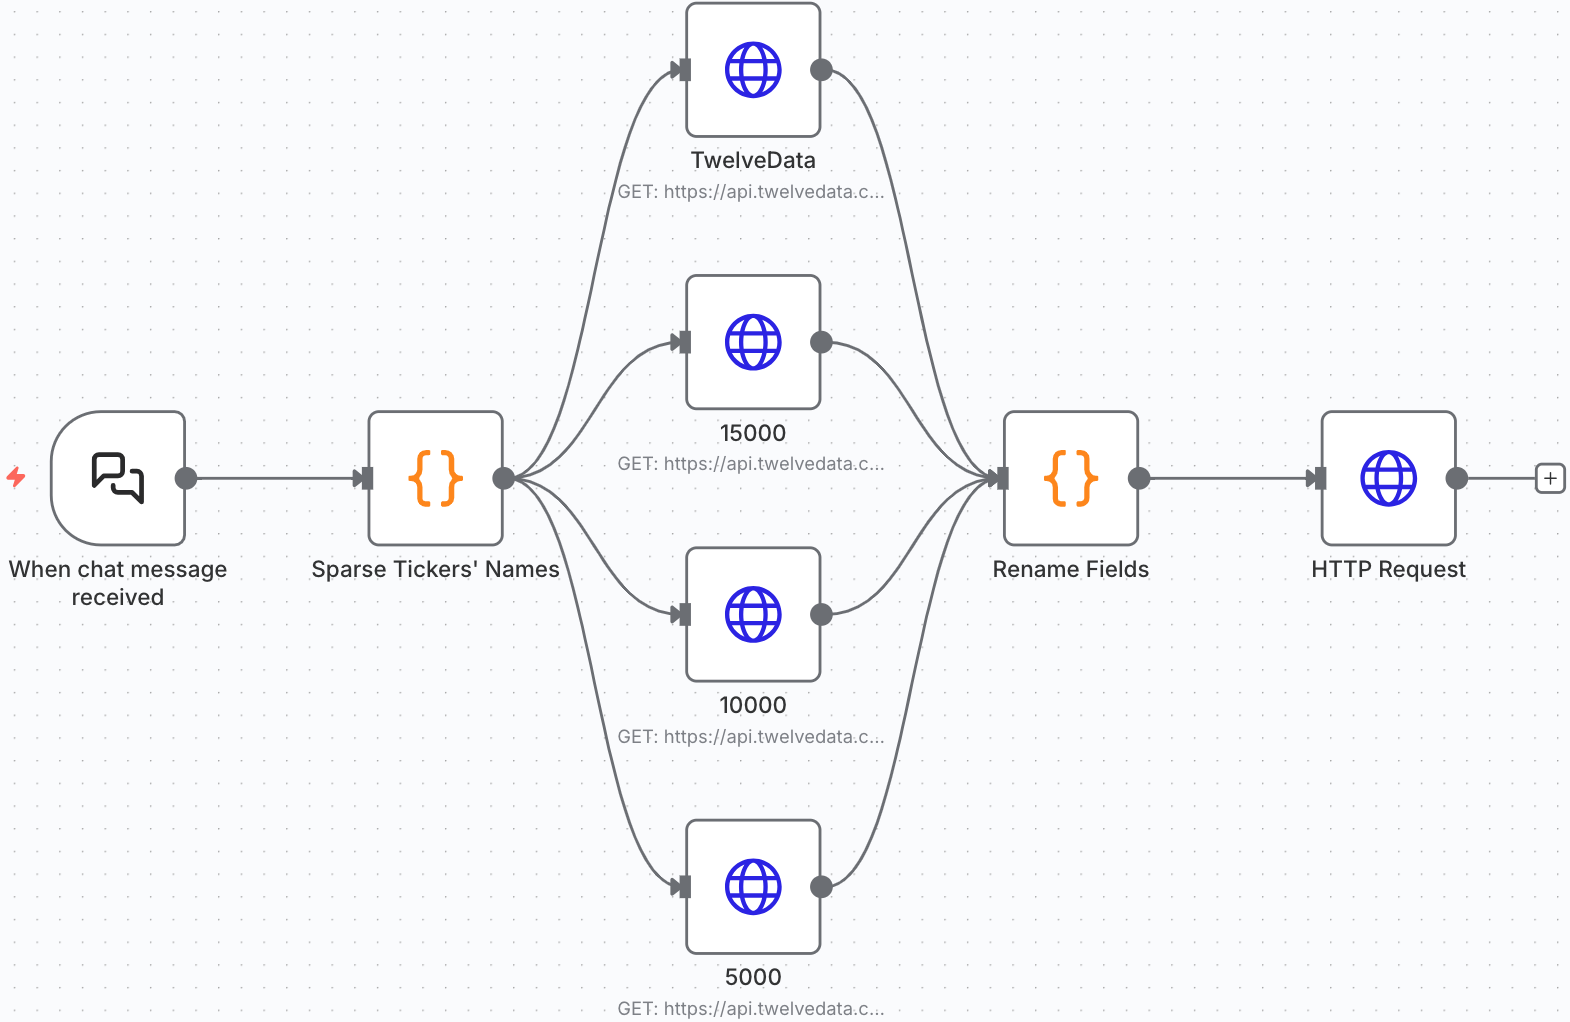
\includegraphics[width=\textwidth]{images/n8n_batch_fetch_diagram.png}
  \caption{n8n Automation Workflow}
  \label{n8n_workflow}
\end{figure}

\vspace{0.5em}
\noindent
The workflow proceeds as follows:
\begin{enumerate}
  \item \textbf{Trigger:} A chat message or scheduled event initiates the workflow, providing a sparse list of ticker symbols.
  \item \textbf{Ticker Parsing:} Splits the input into distinct tickers.
  \item \textbf{Parallel Data Retrieval:} For each ticker, multiple branches issue parallel TwelveData GET requests, each with parameters:
        \begin{itemize}
          \item \texttt{symbol} = ticker symbol (e.g., \texttt{AAPL})
          \item \texttt{interval} = \texttt{"1day"}
          \item \texttt{outputsize} = \texttt{5000}
          \item \texttt{end\_date}/\texttt{offset} adjusted to retrieve the next batch (e.g., 0, 5000, 10000, ...)
        \end{itemize}
  \item \textbf{Field Normalization:} Responses from the API are run through a renaming module to map fields into a canonical OHLCV schema acceptable to \textcolor{blue}{Supabase}.
  \item \textbf{Upload to Supabase:} Processed data are batched and sent as an HTTP request to Supabase's API for upsert (insert/update) in a PostgreSQL OHLCV table. Deduplication logic ensures that records are unique by (\texttt{date}, \texttt{ticker}).
  \item \textbf{Error Handling:} Built-in checks address API rate limits and partial network errors, enabling retries and robust operation.
\end{enumerate}

\noindent
This configuration enables scalable, automated historical data ingestion, deduplication, and updating. Daily updates are handled automatically by the workflow's cron schedule, so the dataset remains current and comprehensive for all modeled stocks.

\begin{figure}[H]
  \centering
  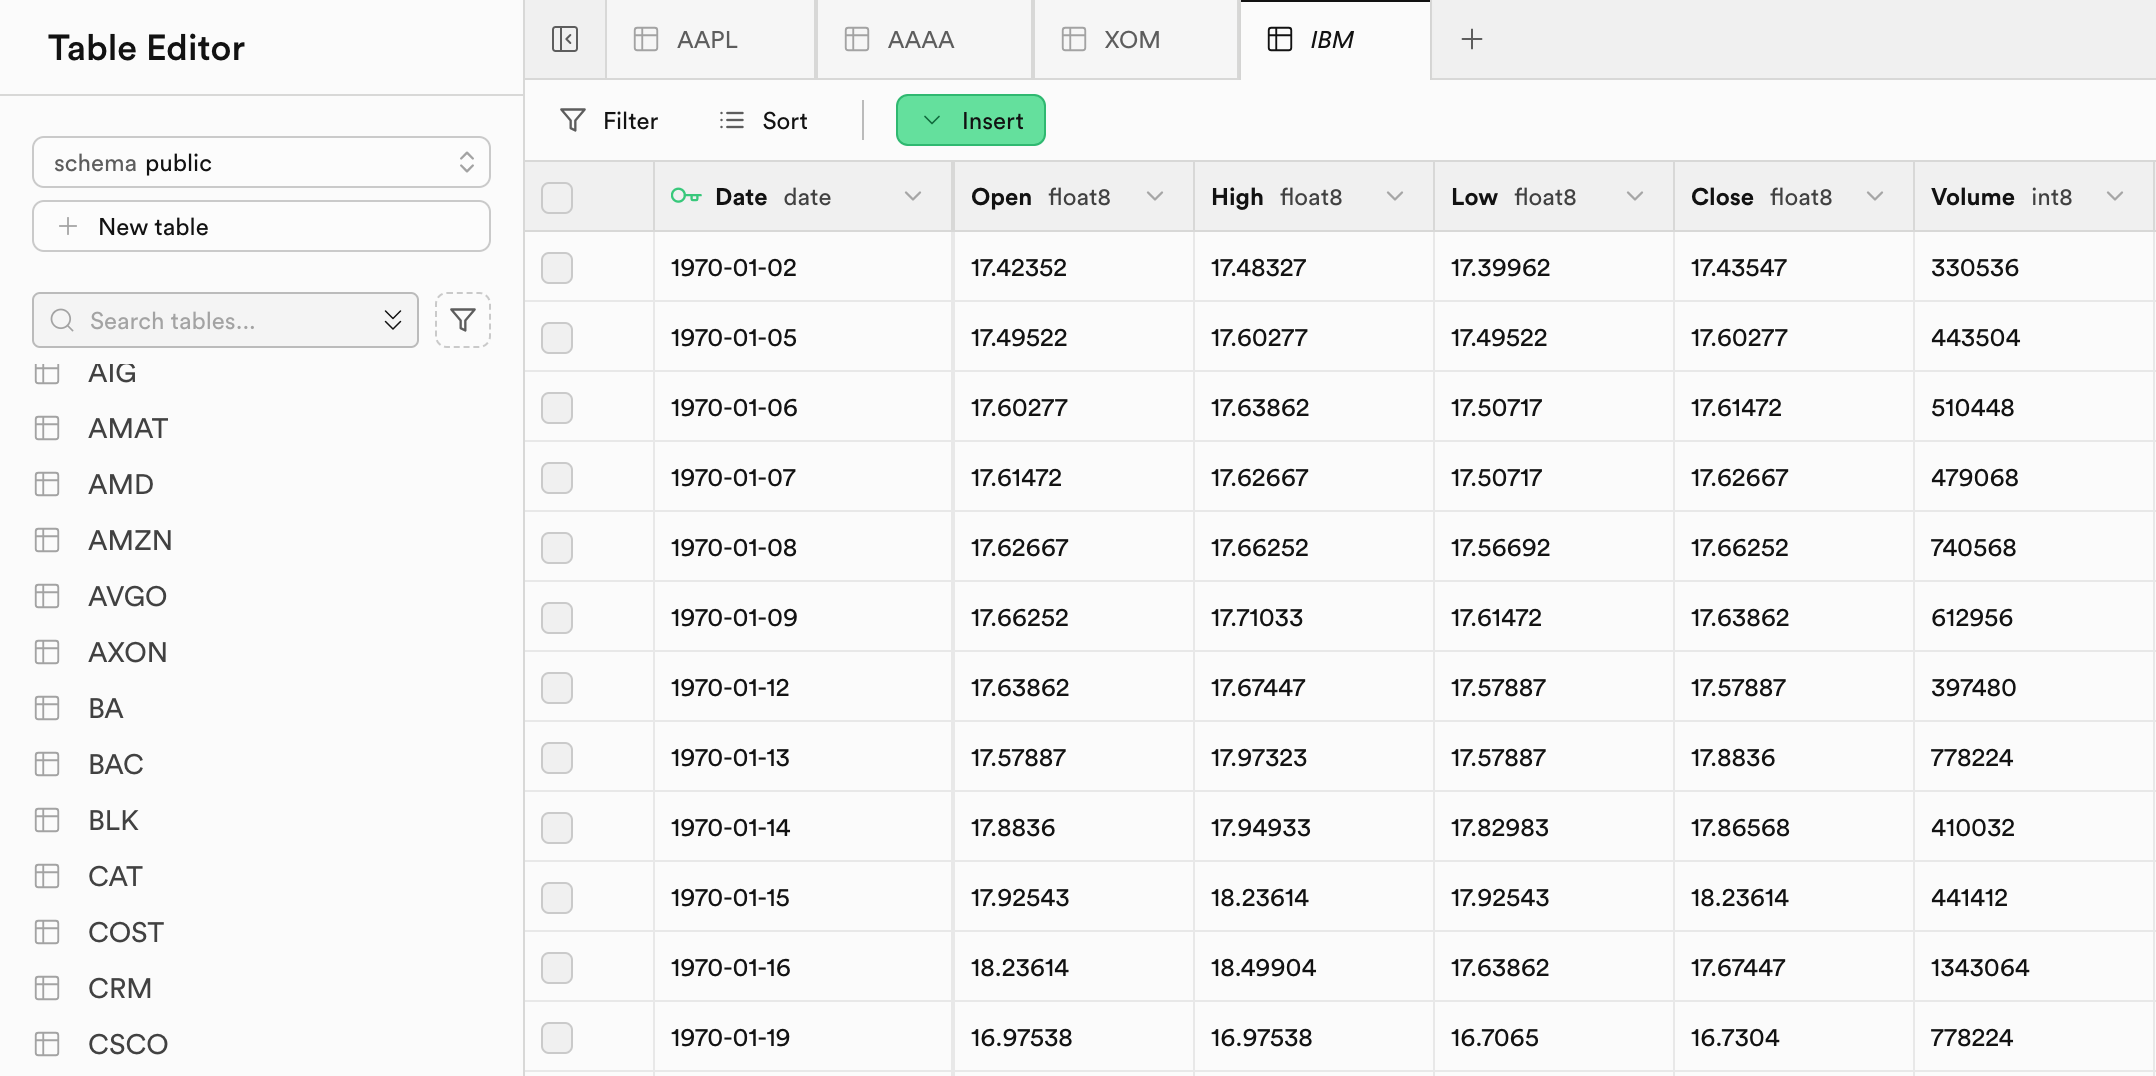
\includegraphics[width=\textwidth]{images/supabase_database.png}
  \caption{Supabase Database}
  \label{supabase_database}
\end{figure}

\subsection{Feature Engineering \& Selection}
The raw OHLCV data is non-stationary and noisy, making it unsuitable for direct deep learning input. I engineered a compact set of six stationary features designed to capture momentum, mean reversion, and volatility regimes.

\subsubsection{Logarithmic Returns (Momentum)}
Logarithmic returns are essential inputs for momentum modeling in financial time series. They are defined by the formula:
\[
  r_t = \ln\left(\frac{P_t}{P_{t-1}}\right)
\]
where $P_t$ denotes the Adjusted Close price at time $t$, and $P_{t-1}$ at the previous time step.

\begin{figure}[H]
  \centering
  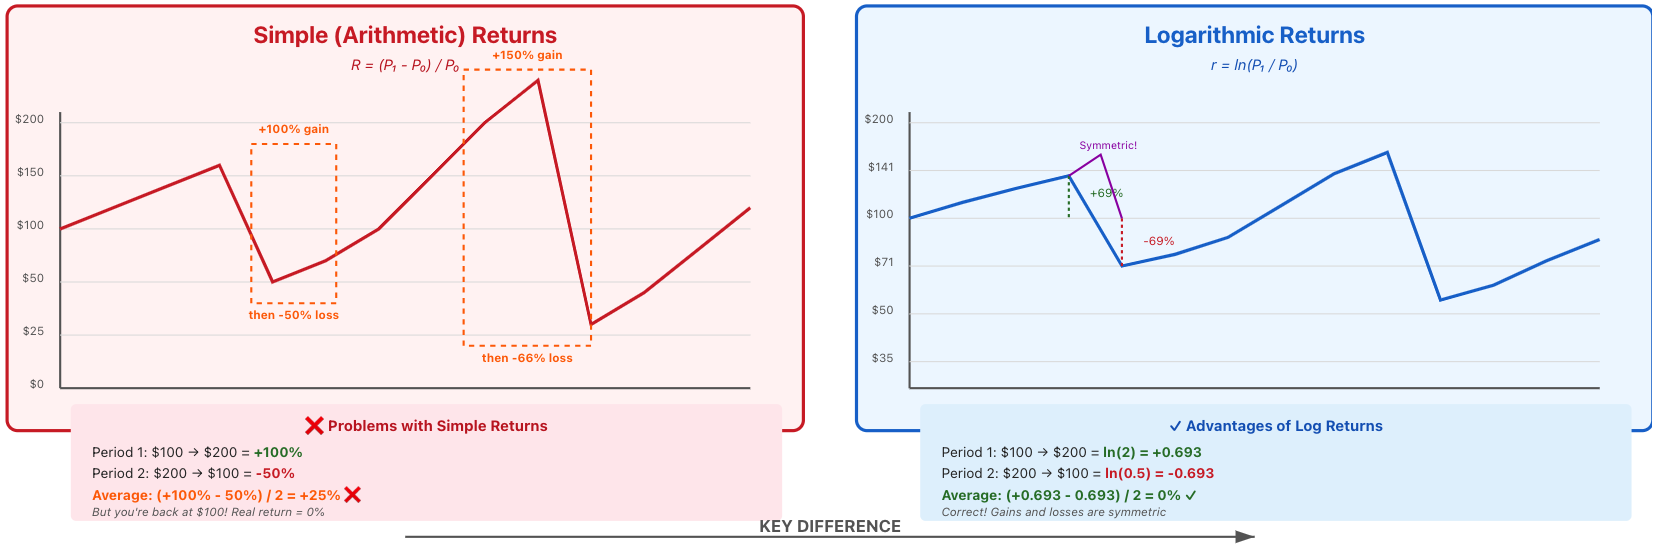
\includegraphics[width=\textwidth]{images/log_return.png}
  \label{log_return}
\end{figure}

Compared to simple arithmetic returns:
\[
  r_t^{(\text{simple})} = \frac{P_t - P_{t-1}}{P_{t-1}}
\]
, log returns possess several important properties:
\begin{itemize}
  \item \textbf{Time Additivity:} Log returns are additive across time intervals, i.e., $\sum_{i=1}^n r_i = \ln\left(\frac{P_n}{P_0}\right)$, enabling aggregation and multi-horizon modeling.
  \item \textbf{Symmetry:} Equal magnitude moves in opposite directions (e.g., $+10\%$ then $-10\%$) symmetrically offset in log space, which stabilizes the statistical properties and aids learning.
  \item \textbf{Statistical Suitability:} Log returns are typically more Gaussian in distribution, which aligns with common output assumptions in probabilistic forecasting models (e.g., Gaussian output heads).
\end{itemize}

Within my experiments, one-day rolling log returns are computed as the change in log Adjusted Close price from $t-1$ to $t$. This serves as the primary input channel to the \textcolor{blue}{LSTM}, enabling the network to model momentum bursts and transient price trends effectively.

\subsubsection{Distance from Moving Averages (Mean Reversion)}
Distance from moving averages is a classic mean reversion feature, quantified as the normalized deviation of the current price from its Simple Moving Average (SMA). Formally, the feature for window $k$ is:

\[
  d_k = \frac{P_t}{\text{SMA}_k(t)} - 1
\]

where $P_t$ is the Adjusted Close price at time $t$ and $\text{SMA}_k(t)$ is the SMA computed over the previous $k$ periods (ending at $t$).

\begin{figure}[H]
  \centering
  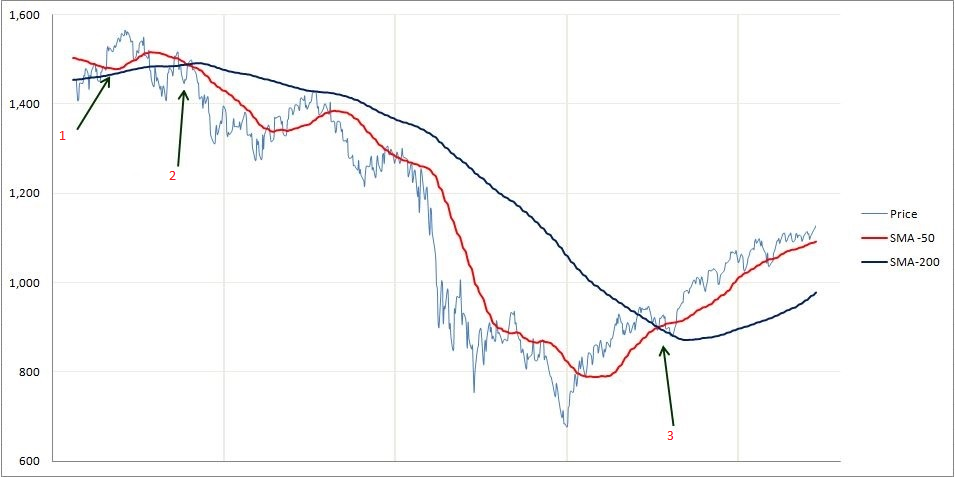
\includegraphics[width=\textwidth]{images/SMA.png}
  \label{SMA}
\end{figure}

I compute this feature for $k \in \{10, 20, 60\}$, providing short-, medium-, and long-term mean reversion signals -- resulting in three feature channels. Financially, assets often exhibit reversion toward their average value: a large positive $d_{60}$ implies the price is far above its long-term mean, potentially indicating overextension (a contrarian sell signal), while a strongly negative $d_{10}$ suggests a recent short-term dip (a potential buy signal).\\

Feeding these distances into the model provides multi-scale contextual information about how unusual the current price is with respect to its recent history, helping the Transformer distinguish genuine breakouts from noisy fluctuations.

\subsubsection{Rolling Volatility (Regime Detection)}
Rolling volatility assists in detecting changes in market regime by quantifying the dispersion of returns. Mathematically, rolling volatility at time $t$ is computed as the standard deviation of log returns over a trailing window:
\[
  \sigma_t = \sqrt{\frac{1}{N-1} \sum_{i=0}^{N-1} (r_{t-i} - \bar{r})^2}
\]
where $r_{t-i}$ are log returns for each of the $N$ most recent time steps and $\bar{r}$ is their mean. For my experiments, I set $N=20$ (roughly one trading month), chosen to balance responsiveness with stability.\\

\begin{figure}[H]
  \centering
  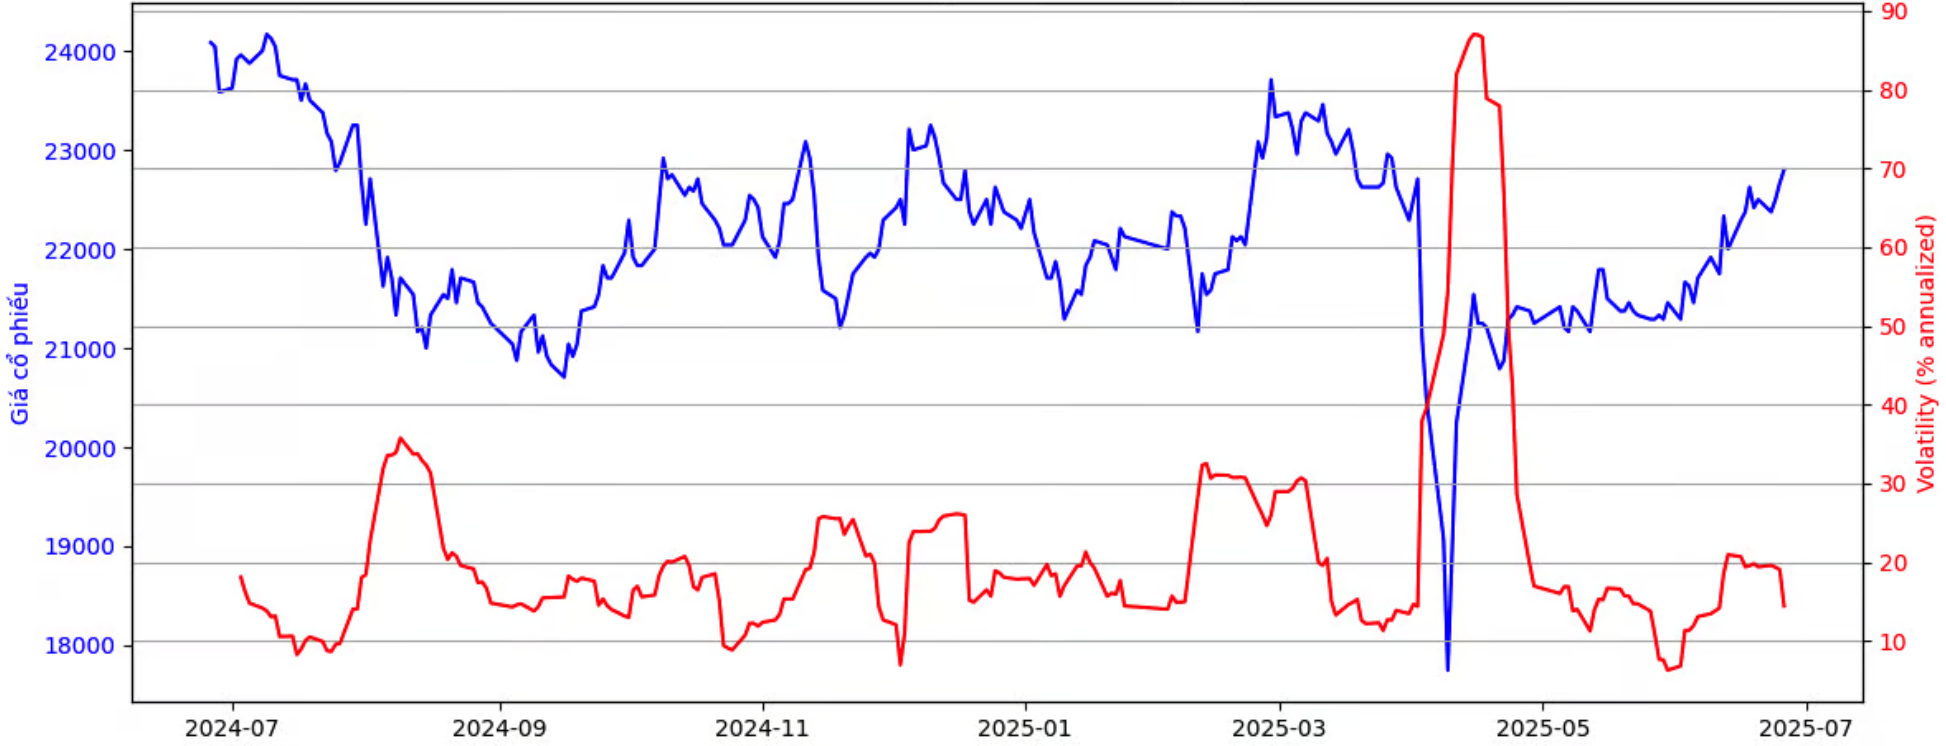
\includegraphics[width=\textwidth]{images/roll_vol.png}
  \label{roll_vol}
\end{figure}

Rolling volatility highlights transitions between "calm" and "turbulent" regimes: extended periods of low $\sigma_t$ typically correspond to stable, mean-reverting markets, while spikes in $\sigma_t$ indicate stress, uncertainty, or trend formation.\\

In model training, this feature feeds into the regime-switching behavior of the output distribution: when input volatility is high, the model is encouraged to predict a larger output standard deviation, yielding appropriately wider confidence intervals. This property is crucial for risk-aware forecasting, as strategies that ignore regime changes typically underperform or fail entirely during volatile periods. Including rolling volatility as an input feature ensures the model can learn to adapt its forecasts to varying market conditions.

\subsubsection{Relative Strength Index (Overbought/Oversold)}
The Relative Strength Index (RSI) is a widely-used momentum oscillator that quantifies the speed and magnitude of recent price changes to identify overbought and oversold conditions. It is computed as:

\[
  RSI_t = 1 - \frac{1}{1 + RS_t}
\]
where
\[
  RS_t = \frac{\text{Average Gain over 14 periods}}{\text{Average Loss over 14 periods}}
\]

\begin{figure}[H]
  \centering
  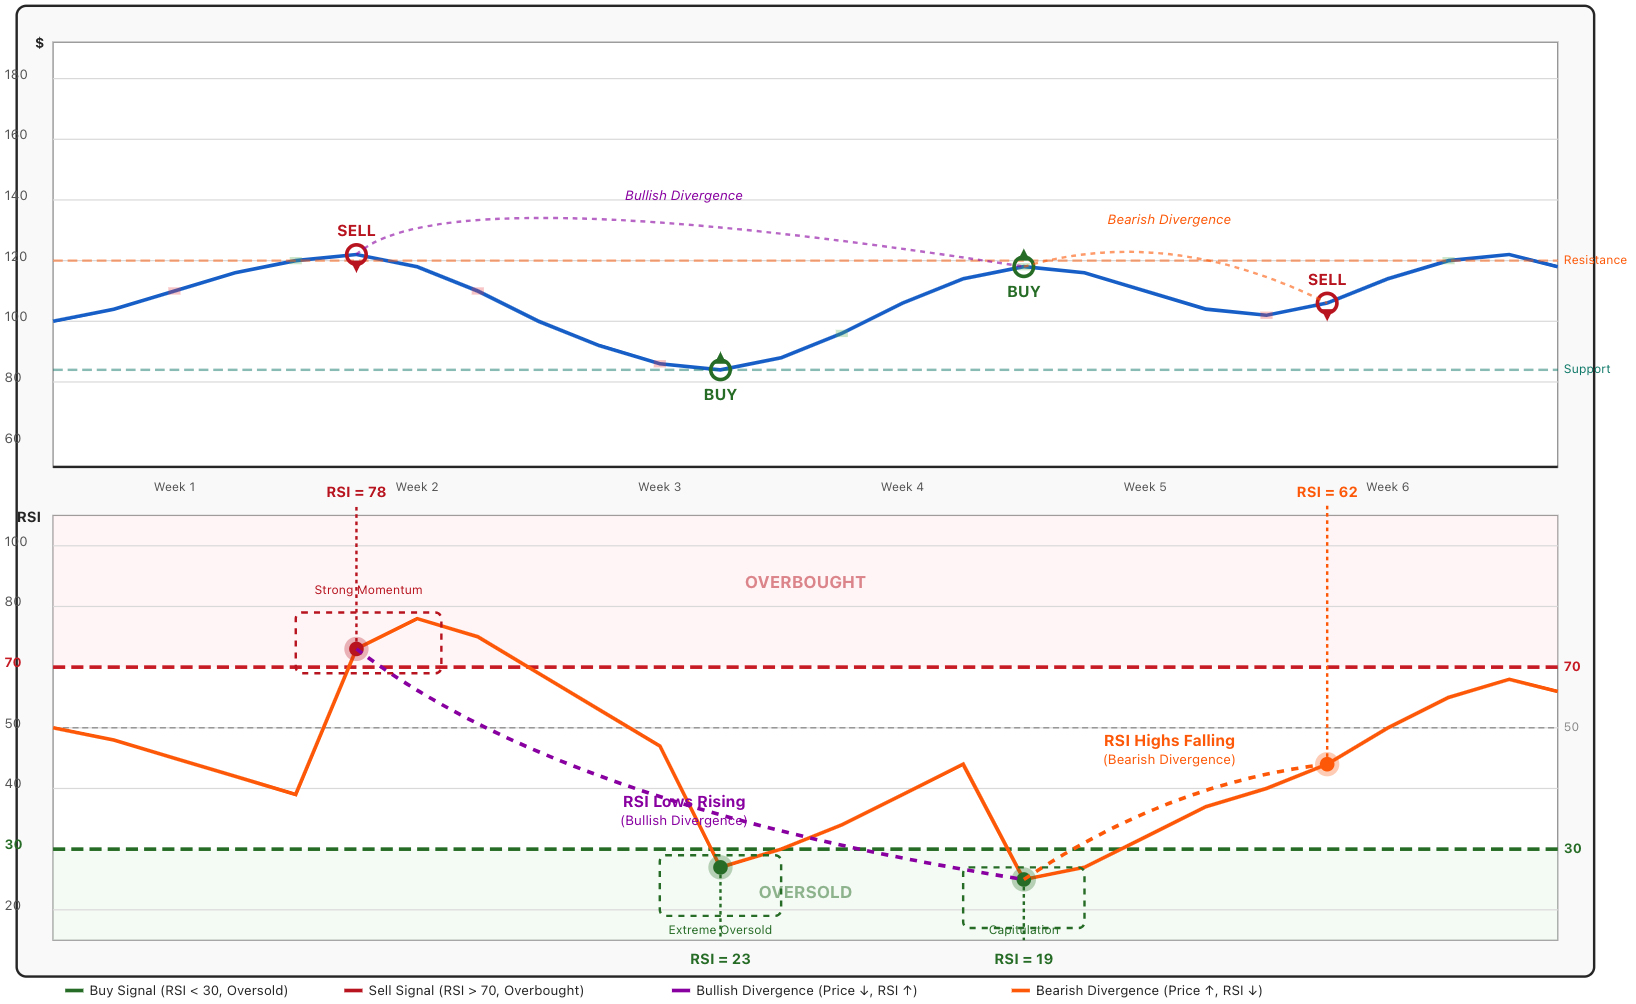
\includegraphics[width=\textwidth]{images/RSI.png}
  \label{RSI}
\end{figure}
This version of RSI is scaled to the $[0, 1]$ range (as opposed to the traditional $[0, 100]$), which normalizes it for model input. For modeling, a standard lookback window of 14 days is used.\\

High RSI values ($>$ 0.7) indicate an overbought regime where price rises may be exhausted, while low values ($<$ 0.3) suggest oversold conditions, potentially flagging a reversal. By incorporating RSI alongside log returns in the feature set, the model can better distinguish between sustainable price momentum and unsustainable, exhausted moves, thereby reducing the likelihood of false signals around local extremes.

\subsubsection{Cross-Sectional Normalization (The "Alpha" Layer)}
\label{section_3.3.5}
Finally, cross-sectional normalization forms the "Alpha" layer, applied to all features across the universe of stocks for each day. The normalization is defined as:
\[
  z_{i, t} = \frac{x_{i, t} - \mu_t}{\sigma_t}
\]
where $x_{i, t}$ is the raw feature value for stock $i$ at time $t$, $\mu_t$ is the cross-sectional mean of that feature across all $N$ stocks at time $t$, and $\sigma_t$ is the corresponding standard deviation:
\[
  \mu_t = \frac{1}{N} \sum_{i=1}^N x_{i, t}, \qquad
  \sigma_t = \sqrt{ \frac{1}{N} \sum_{i=1}^N (x_{i, t} - \mu_t)^2 }
\]

\begin{figure}[H]
  \centering
  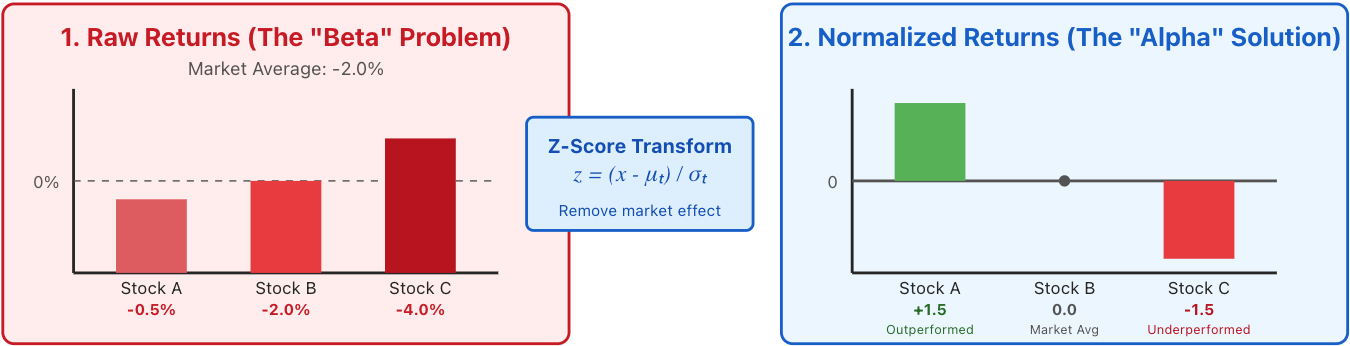
\includegraphics[width=\textwidth]{images/alpha.png}
  \label{alpha}
\end{figure}

This normalization is performed \textit{across} the stock universe for each feature and timestep, removing common market-wide effects (the ``Beta'' component) and making all features ``relative'' rather than absolute. For example, if the overall market drops sharply and every stock suffers negative returns, Z-score normalization will center and standardize these values. A stock that declines \textit{less} than average (e.g., $-2\%$ when the average is $-5\%$) will achieve a positive $z_{i, t}$, highlighting \textit{relative} outperformance despite an absolute loss.\\

This approach directly aligns with cross-sectional ranking objectives: the model is incentivized to learn patterns of relative strength and weakness, rather than predicting the absolute direction or magnitude of future returns. As a result, forecasting focuses on correctly ranking stocks by their likely performance, which matches the requirements of objectives like \textcolor{blue}{MarginRankingLoss} and typical quantitative investment strategies. By normalizing all features in this way prior to input, the model becomes robust to shifts in broad market conditions and can identify the stocks most likely to outperform their peers in any environment.
\clearpage
\begin{lstlisting}[language=Python]
def _engineer_features(self, df):
  df = df.copy()
  df['Log_Ret'] = np.log(df['Close'] / df['Close'].shift(1)) 
  df['Log_Ret_Raw'] = df['Log_Ret']
  df['Target_5D'] = df['Log_Ret_Raw'].rolling(window=CONFIG['pred_horizon'])
                    .sum().shift(-CONFIG['pred_horizon'])
  
  for p in [10, 20, 60]:
    sma = df['Close'].rolling(p).mean()
    df[f'Dist_SMA_{p}'] = (df['Close'] / sma - 1)
      
  df['Vol_20'] = df['Log_Ret'].rolling(20).std()
  
  delta = df['Close'].diff()
  gain = (delta.where(delta > 0, 0)).ewm(span=14).mean()
  loss = (-delta.where(delta < 0, 0)).ewm(span=14).mean()
  rs = gain / loss.replace(0, 1e-9)
  df['RSI'] = (100 - (100 / (1 + rs))) / 100.0
  return df.dropna()
\end{lstlisting}

\subsection{Constructing Universal Stock Dataset}
\subsubsection{Panel Alignment \& Cleaning}
To construct a cohesive multi-stock dataset from individual ticker files, the raw DataFrames were concatenated into a master panel. Crucially, specifically for the Cross-Sectional Transformer layer to operate on consistent tensor dimensions ($N_{stocks} \times L_{seq} \times D_{feat}$) without the need for complex masking or padding -- which could distort attention weights—a strict balanced panel was enforced. This involved retaining only trading dates containing complete OHLCV records across all 53 tickers. This alignment strategy, achieved by grouping by date and verifying ticker counts, yielded approximately 1,420 valid trading days (from Jan 2020).\\

The rationale involves both engineering efficiency and statistical validity: incomplete data introduces artifacts that bias the daily cross-sectional Z-score normalization \result{Section~\ref{section_3.3.5}}, while a fixed universe ensures the model learns true inter-stock dynamics (e.g., sector rotation) within a consistent market context, ensuring computational stability for the attention mechanism.

\subsubsection{Tensor Normalization \& Clipping}
Shifting from absolute to relative predictions, daily Z-score normalization was applied cross-sectionally:
\[
  x_{i,t}^{\text{norm}} = \frac{x_{i,t} - \mu_t}{\sigma_t + \epsilon}
\]
where $x_{i,t}$ is the value of a given feature for stock $i$ on day $t$, $\mu_t$ is the mean of that feature across all 53 stocks for day $t$, and $\sigma_t$ is the corresponding standard deviation (with a small $\varepsilon$ added for numerical stability). After normalization, values were clipped to the range $[-3,\, 3]$ to mitigate the effect of extreme outliers.\\

This cross-sectional normalization effectively removes market ``beta'' -- the common movement of stocks during broad rallies or sell-offs -- and isolates the ``alpha'' component, i.e., stock-specific outperformance or underperformance relative to the peer group. Without this step, raw features would bias the model to forecast general market direction, undermining its ability to distinguish winners from losers.\\

Crucially, this normalization aligns the input distribution with the \texttt{\textcolor{blue}{MarginRankingLoss}} objective, which trains the model to order stocks by expected performance rather than absolute magnitude. This synergy makes alpha extraction feasible and results in robust cross-sectional metrics; specifically, my experiments demonstrate Information Coefficient (IC) values reaching 0.0797 (See \result{Picture~\ref{IC}}), significantly exceeding the standard industry threshold of 0.03 (See \result{Table~\ref{tab:hyperparameter_value}}) and highlighting the model's capability to identify relative outperformance regardless of the prevailing market regime.

\subsubsection{Tensor Construction for Hybrid Processing}
The \texttt{UniversalDataset} organizes the panel hierarchically by date and stock identifier, facilitating efficient tensorization tailored for the hybrid architecture. For each prediction timestamp, the system assembles a comprehensive market snapshot: a 60-day rolling window across the entire universe, yielding a tensor of shape $\mathbf{X} \in \mathbb{R}^{N \times T \times D}$, where $N=53$ (stocks), $T=60$ (sequence length), and $D$ is the feature dimension.

This structured tensor enables a dual-stage computational workflow:
\begin{enumerate}
  \item \textbf{Temporal Encoding:} The \textcolor{blue}{LSTM} layers in \result{Section~\ref{section_4.1.1}} process the $T$-dimension independently for each stock, encoding idiosyncratic historical patterns into latent embeddings.
  \item \textbf{\textcolor{blue}{Cross-Sectional Attention}:} Subsequently, the Transformer in \result{Section~\ref{section_4.1.2}} applies attention across the $N$-dimension (batch) at the specific prediction day, explicitly modeling inter-stock dependencies and sector relationships.
\end{enumerate}

\begin{lstlisting}[language=Python]
class UniversalDataset(Dataset):
  def __init__(self, df, feature_cols, seq_len, num_stocks):
    self.df = df.sort_values(['Date', 'Stock_ID']) # Crucial Sort
    self.feature_cols = feature_cols
    self.seq_len = seq_len
    self.num_stocks = num_stocks
    
    self.dates = sorted(df['Date'].unique())
    self.date_to_idx = {date: i for i, date in enumerate(self.dates)}
    self.valid_dates = self.dates[self.seq_len:]

  def __len__(self):
    return len(self.valid_dates)

  def __getitem__(self, idx):
    date = self.valid_dates[idx]
    window_start = self.date_to_idx[date] - self.seq_len + 1
    window_dates = self.dates[window_start : self.date_to_idx[date] + 1]
    # Fast slice because df is sorted by Date
    window_df = self.df[self.df['Date'].isin(window_dates)]
    # Check integrity
    if len(window_df) != self.seq_len * self.num_stocks:
      # Fallback for edge cases (though "Fixed Universe" prevents this)
      x = torch.zeros(self.num_stocks, self.seq_len, len(self.feature_cols))
    else:
      # Shape: [Seq_Len * Stocks, Features]
      flat = window_df[self.feature_cols].values.astype(np.float32)
      # Reshape: [Seq_Len, Stocks, Features]
      x = flat.reshape(self.seq_len, self.num_stocks, -1)
      # Transpose: [Stocks, Seq_Len, Features]
      x = np.transpose(x, (1, 0, 2))
      x = torch.FloatTensor(x)
    
    stock_ids = torch.arange(self.num_stocks)
    y = window_df[window_df['Date'] == date]['Target_5D'].values.astype(np.float32)
    
    return x, stock_ids, torch.FloatTensor(y)
\end{lstlisting}

To ensure rigorous evaluation, the dataset employs a strict chronological split (80\% training, 20\% hold-out testing) as implemented in the data loader. This approach eliminates look-ahead bias and supports robust out-of-sample validation. Ultimately, this tensor-centric design not only maximizes GPU parallelism but also allows the model to generate fully contextualized, uncertainty-calibrated forecasts -- directly supporting practical, low-turnover portfolio signals.

\section{Model Implementation}
\subsection{Model Architecture}
The hybrid deep learning architecture is designed to process 60-day sequences of cross-sectionally normalized features, producing probabilistic 5-day interval predictions. This system integrates temporal sequence modeling with cross-sectional contextualization, leveraging a Gaussian output head for uncertainty quantification. By focusing on a fixed universe of 53 stocks, the model emphasizes alpha capture through relative rankings, addressing the stochastic nature of financial markets.

\subsubsection{Temporal Encoder (\textcolor{blue}{LSTM})}
\label{section_4.1.1}
The temporal extraction phase begins with a 2-layer Long Short-Term Memory (\textcolor{blue}{LSTM}) network designed to isolate stock-specific momentum and mean-reversion signals before cross-sectional interaction occurs. The encoder is configured with a hidden dimension of 128 units and operates in a unidirectional, batch-first manner.\\

For every stock $i$ in the universe, the \textcolor{blue}{LSTM} processes the input sequence $\mathbf{X}_i \in \mathbb{R}^{60 \times D}$, where $D$ represents the engineered feature set (log returns, volatility, RSI, and distances to simple moving averages). The recurrence relation is defined as $h_t = \mathrm{\textcolor{blue}{LSTM}}(x_t, h_{t-1})$, effectively compressing the 60-day historical window into a latent state vector.

\begin{itemize}
  \item \textbf{Hierarchical Feature Extraction:} The 2-layer stacking allows the network to learn at different temporal resolutions: lower layers capture high-frequency noise and transient momentum pulses, while upper layers abstract longer-term trends.
  \item \textbf{Regularization:} To mitigate overfitting given the noisy financial data, a Dropout rate of approximately 0.44 (specifically 0.4395 in the optimized configuration) is applied between \textcolor{blue}{LSTM} layers.
\end{itemize}

The final hidden state of the last time step, $h_{60} \in \mathbb{R}^{128}$, serves as the distinct temporal embedding for each stock. This design creates a bottleneck that forces the model to distill the most salient historical drivers into a fixed-size vector, which is subsequently passed to the Context Layer for cross-sectional comparison.

\begin{figure}[H]
  \centering
  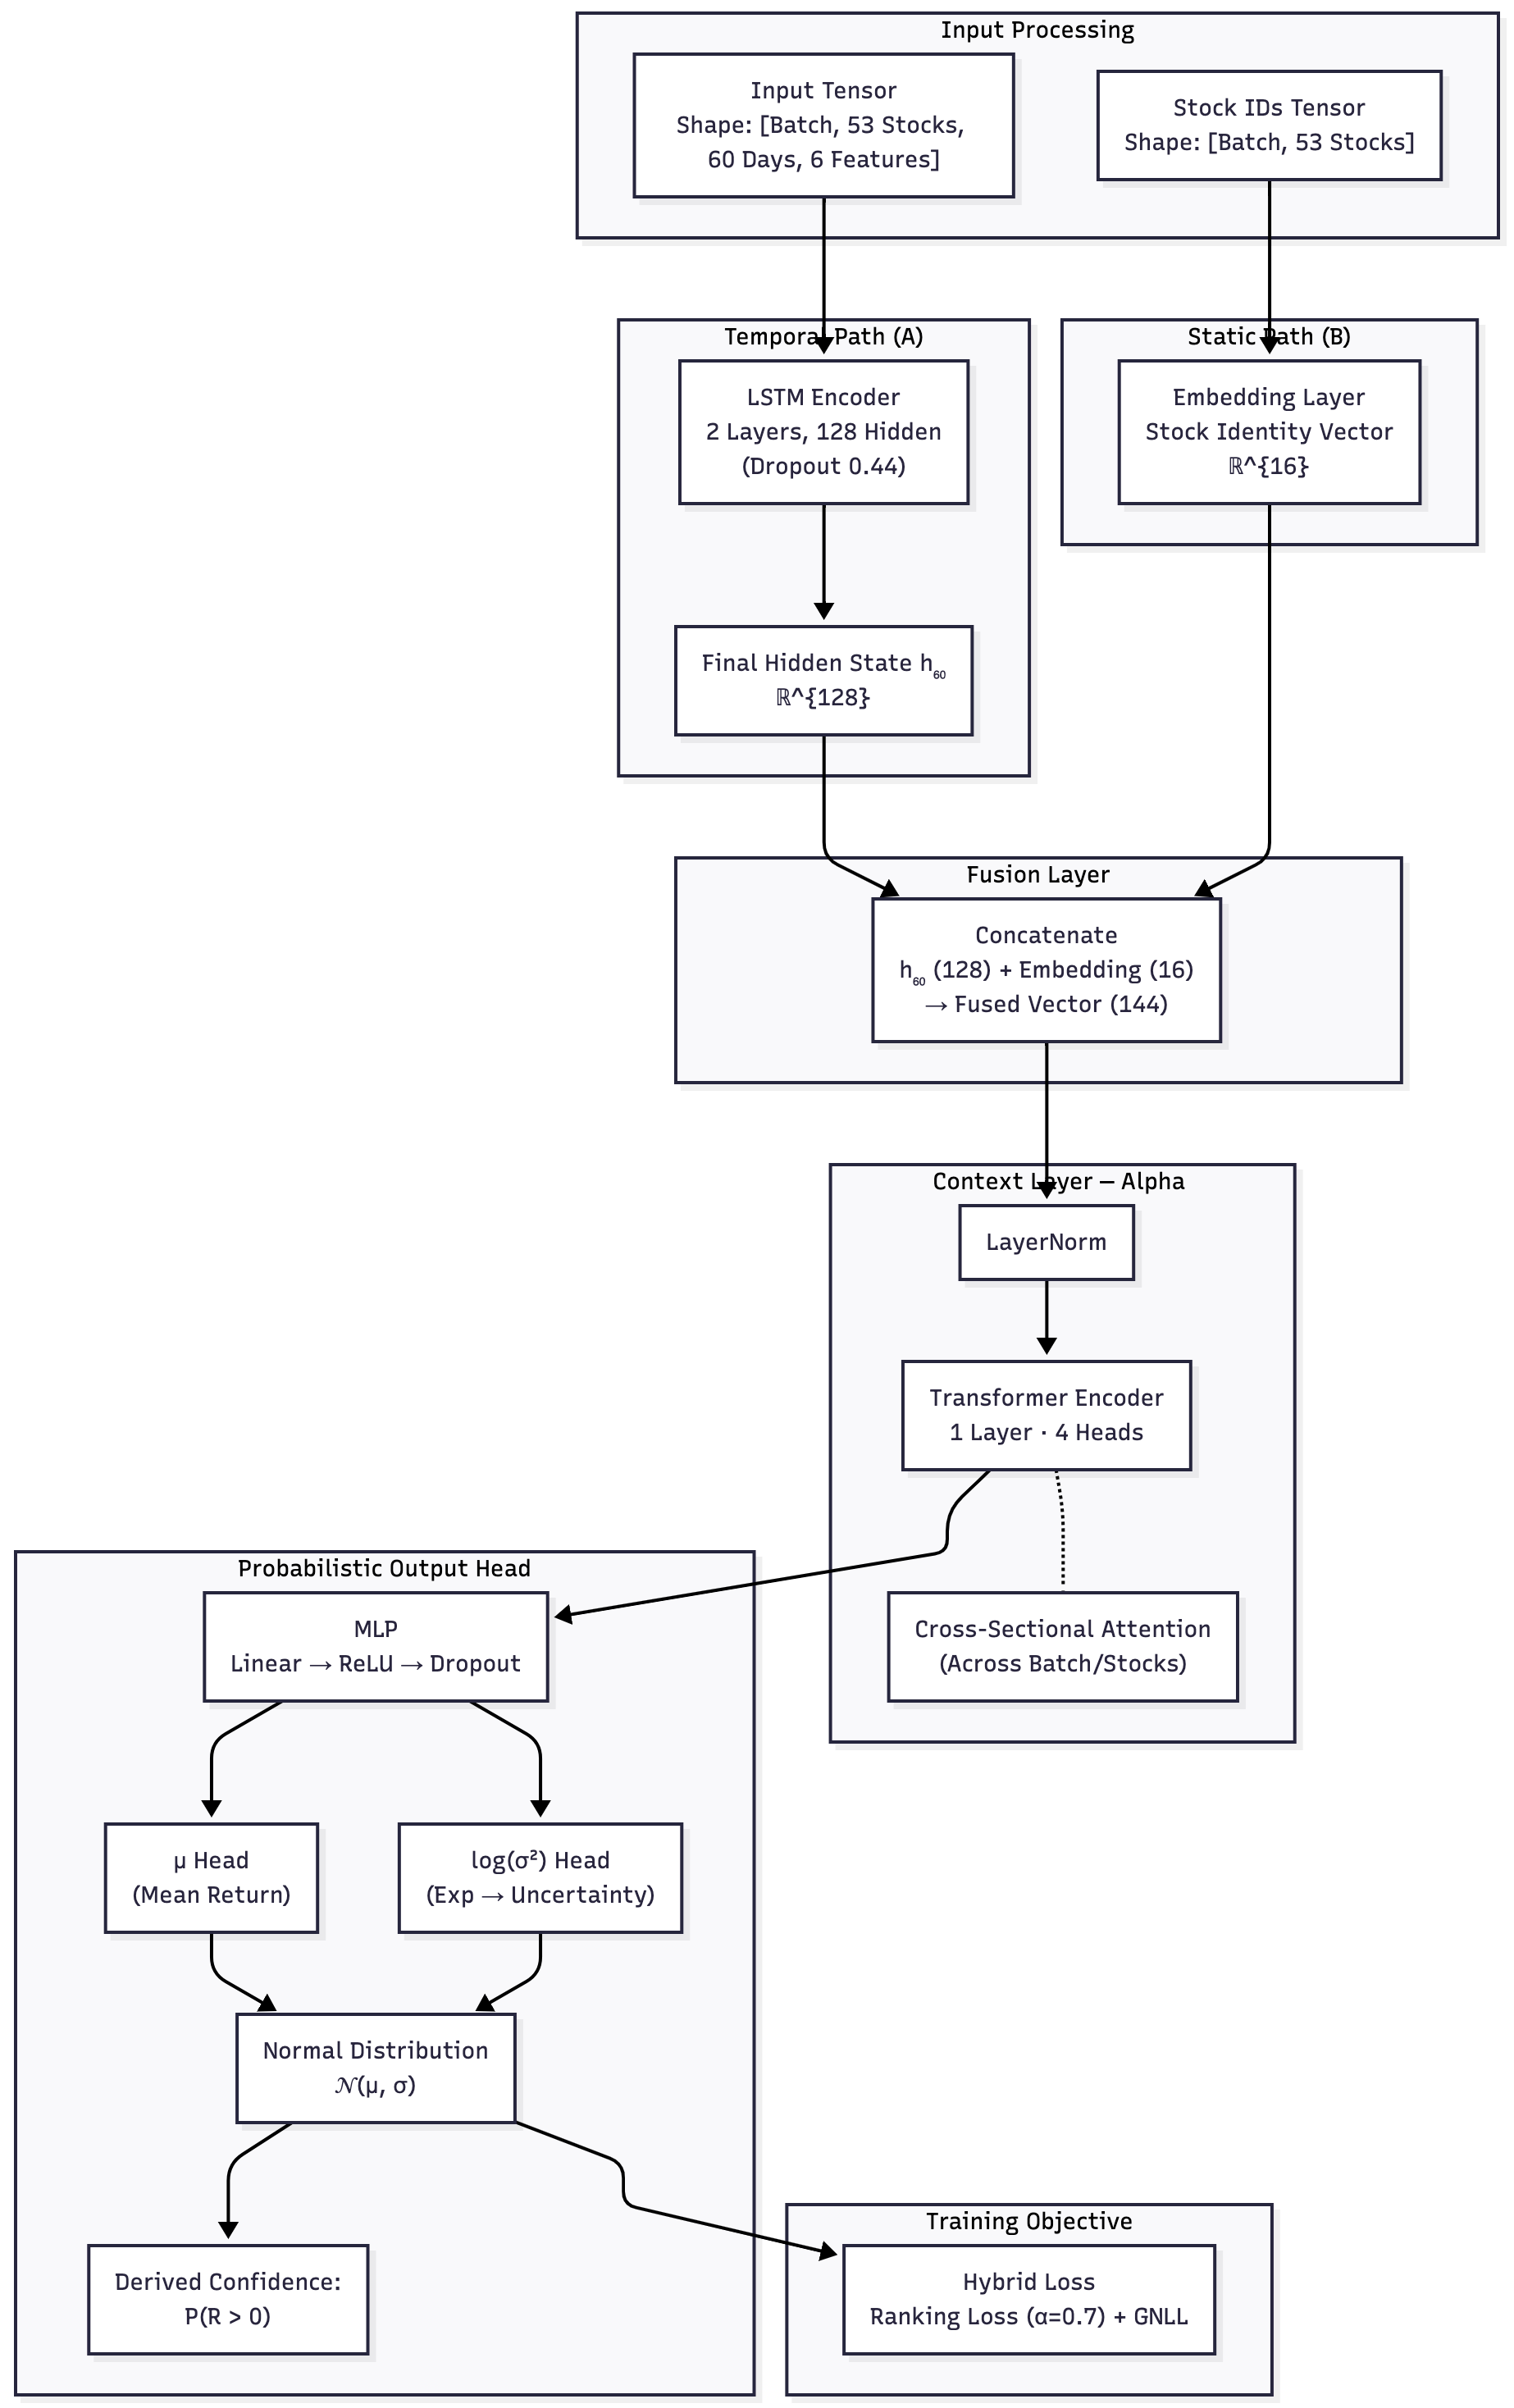
\includegraphics[width=0.85\textwidth]{images/model_architecture.png}
  \caption{Model Architecture}
  \label{model_architecture}
\end{figure}

\subsubsection{Context Layer (Cross-Sectional Transformer)}
\label{section_4.1.2}
To infuse inter-stock contextual awareness -- such as sector correlations or relative momentum -- the model employs a cross-sectional Transformer mechanism. First, the \textcolor{blue}{LSTM}'s final hidden state ($h_{60}$, 128 dimensions) is concatenated with a learnable stock identity embedding (16 dimensions), forming a fused vector of 144 dimensions. This fusion integrates idiosyncratic temporal dynamics with static stock-specific traits.\\

The combined vector undergoes Layer Normalization for stabilization, then enters a 2-layer Transformer Encoder with 4 attention heads. Crucially, while the model is trained on mini-batches of randomized days (e.g., $B=128$) to ensure robust optimization, the Attention mechanism operates across the stock universe dimension ($N=53$). For every individual market snapshot (day) within the batch, the Transformer treats the list of 53 stocks as the sequence context. This allows each stock's representation to attend to every other stock in the universe contemporaneously. For instance, the query for a technology stock can weigh keys and values from financial sector peers, capturing phenomena like sector rotation or capital flow shifts.\\

Dropout is applied within the Transformer to enhance generalization. This layer's output refines the latent features, enabling the model to adjust predictions based on the holistic market state relative to peers. This architecture directly supports alpha isolation and ranking accuracy, yielding outcomes like the Golden Model's high IC, where inter-stock learning boosts ordinal predictions without temporal dilution.

\subsubsection{Probabilistic Head}
Following cross-sectional contextualization, the refined latent representations are projected through a Probabilistic Multi-Layer Perceptron (MLP) head. This component translates the high-dimensional context vectors into actionable distributional parameters, explicitly addressing the heteroscedastic nature of financial returns.\\

The MLP reduces the dimensionality via a linear layer to 32 units, followed by a ReLU activation and a second Dropout layer for regularization. The final output layer projects this vector into two distinct scalars for each stock:

\begin{enumerate}
  \item $\mu$ (Conditional Mean): The expected 5-day cumulative log return.
  \item $\log(\sigma^2)$ (Log Variance): A learned uncertainty parameter.
\end{enumerate}

Using $\log(\sigma^2)$ ensures numerical stability and guarantees positivity when converted to standard deviation via exponentiation ($\sigma = \exp(0.5 \times \log \sigma^2)$). This parametrizes a Gaussian predictive distribution $\mathcal{N}(\mu, \sigma)$ for every stock. By learning variance end-to-end via the \texttt{GaussianNLLLoss}, the model is incentivized to widen its confidence intervals during volatile market regimes (high uncertainty) and narrow them during stable trends. This mechanism is critical for the resulting low turnover (See \result{Table~\ref{tab:backtest_metrics}}), as it naturally suppresses trading signals when the model detects low-confidence regimes.

\subsubsection{Confidence Derivation}
\label{section_4.1.4}
A key advantage of the probabilistic architecture is the ability to derive an analytical confidence score without additional model complexity. Rather than relying on a raw regression scalar, the strategy computes the probability of a positive return, $P(R > 0)$, using the Cumulative Distribution Function (CDF) of the predicted Normal distribution:
\[
  P(R > 0) = 1 - \Phi\left( \frac{0 - \mu}{\sigma} \right)
\]
where $\Phi$ is the standard Normal CDF, $\mu$ is the predicted return, and $\sigma$ is the predicted volatility. This formula calculates the area under the probability density curve that lies above zero.\\

This derivation transforms the model's raw output into an interpretable risk metric (e.g., ``75\% probability of profit''). In the ``Golden Model'' backtest, this score acts as a rigorous filter -- positions are only taken when confidence exceeds a specific threshold. This selective engagement directly contributed to the high Sortino Ratio of 2.29, effectively permitting the strategy to remain cash-heavy during uncertain drawdowns while aggressively capitalizing on high-conviction opportunities.

\begin{lstlisting}[language=Python]
class AdvancedCrossSectionalModel(nn.Module):
  def __init__(self, num_stocks, input_dim, hidden_dim, embed_dim, num_heads, dropout):
    super().__init__()
    self.embedding = nn.Embedding(num_stocks, embed_dim)
    self.\textcolor{blue}{LSTM} = nn.\textcolor{blue}{LSTM}(
        input_dim, hidden_dim, num_layers=2, batch_first=True, dropout=dropout
    )
    # Transformer for Cross-Sectional Attention
    d_model = hidden_dim + embed_dim
    self.norm = nn.LayerNorm(d_model) # Stabilizer
    self.transformer = nn.TransformerEncoderLayer(
        d_model=d_model, nhead=num_heads, dropout=dropout, batch_first=True
    )
    self.head = nn.Sequential(
        nn.Linear(d_model, 32),
        nn.ReLU(),
        nn.Dropout(dropout),
        nn.Linear(32, 2) 
    )
      
  def forward(self, x, stock_ids):
    b, s, seq, f = x.shape
    
    x_flat = x.view(b * s, seq, f)
    lstm_out, _ = self.\textcolor{blue}{LSTM}(x_flat)
    last_step = lstm_out[:, -1, :] # [B*S, Hidden]
    
    if stock_ids.dim() == 1:
      stock_ids = stock_ids.repeat(b, 1)
    ids_flat = stock_ids.view(b * s)
    embeds = self.embedding(ids_flat)
    # Cross-Sectional Attention
    combined = torch.cat([last_step, embeds], dim=1) # [B*S, D_Model]
    # Reshape for Transformer: [Batch, Stocks, D_Model]
    combined_view = combined.view(b, s, -1)
    combined_norm = self.norm(combined_view)
    # Attend across stocks in the same batch (day)
    attended = self.transformer(combined_norm) # [Batch, Stocks, D_Model]
    # Prediction Head
    out = self.head(attended) # [Batch, Stocks, 2]
    return out[:, :, 0], out[:, :, 1] # Mu, Log_Var
\end{lstlisting}

\subsection{Optimization \& Loss Function}

To balance the dual objectives of accurate ordinal ranking (\textbf{Alpha}) and calibrated uncertainty estimation (\textbf{Risk}), the model is trained using a composite objective function optimized via the AdamW algorithm. The optimization dynamics -- including learning rate and weight decay -- are tuned via the Bayesian search described in \result{Section ~\ref{section_4.3}}, ensuring stable cooperation between the \textcolor{blue}{LSTM} and Transformer modules.

\paragraph{Hybrid Loss Function}
The total loss $\mathcal{L}$ is a convex combination of two components, governed by a weighting hyperparameter $\alpha$:

\[
  \mathcal{L} = \alpha \cdot \mathcal{L}_{\mathrm{Rank}} + (1-\alpha) \cdot \mathcal{L}_{\mathrm{GNLL}}
\]

\begin{enumerate}
  \item \textbf{Ranking Component ($\mathcal{L}_{\mathrm{Rank}}$):} To optimize for cross-sectional ordering -- critical for long-short strategies -- I use the margin ranking loss on pairs of stocks $(i, j)$ in the same batch:
        \[
          \mathcal{L}_{\mathrm{Rank}} = \frac{1}{N_{\mathrm{pairs}}}\sum_{i, j}
          \max\left(0,\, m - (\hat{y}_i - \hat{y}_j) \cdot \mathrm{sign}(y_i - y_j) \right)
        \]
        Here, $y$ denotes the ground-truth return, $\hat{y}$ the predicted mean ($\mu$), and $m$ is a small margin (set to $10^{-4}$). This loss penalizes the model when it misorders stocks -- that is, when $\hat{y}_i < \hat{y}_j$ but actually $y_i > y_j$. Crucially, this digitizes the "Alpha" signal: only relative ordering -- not absolute market direction -- affects this term.

  \item \textbf{Uncertainty Component ($\mathcal{L}_{\mathrm{GNLL}}$):} To calibrate the risk head, I deploy the \textcolor{blue}{Gaussian Negative Log-Likelihood} (GNLL) loss, interpreting model outputs as the mean ($\mu$) and variance ($\sigma^2$) of a normal distribution for each stock:
        \[
          \mathcal{L}_{\mathrm{GNLL}} = \frac{1}{2} \sum_{i} \left(
          \log(2\pi\sigma_i^2) + \frac{(y_i - \mu_i)^2}{\sigma_i^2}
          \right)
        \]
        If the predicted mean is inaccurate, the model can mitigate loss by increasing $\sigma_i^2$, thereby “admitting” uncertainty in difficult regimes; in stable regimes, the $\log(\sigma_i^2)$ term encourages sharper, tighter confidence intervals.
\end{enumerate}

\begin{lstlisting}[language=Python]
class HybridLoss(nn.Module):
  def __init__(self, alpha=0.7, margin=1e-4):
    super().__init__()
    self.alpha = alpha
    self.margin = margin
    self.gnll = nn.GaussianNLLLoss()
      
  def forward(self, mu, log_var, target):
    gnll_loss = self.gnll(mu.flatten(), target.flatten(), torch.exp(log_var.flatten()))
    
    mu_diff = mu.unsqueeze(2) - mu.unsqueeze(1)
    target_diff = target.unsqueeze(2) - target.unsqueeze(1)
    target_sign = torch.sign(target_diff)
    
    loss_matrix = torch.relu(-target_sign * mu_diff + self.margin)
    mask = (target_sign != 0)
    rank_loss = (loss_matrix * mask).sum() / mask.sum().clamp(min=1)
    
    return (1 - self.alpha) * gnll_loss + self.alpha * rank_loss
\end{lstlisting}

\paragraph{Rationale for the Hybrid Approach}
Blending these objectives resolves a fundamental conflict in quantitative finance: regression-only losses (like GNLL) often encourage overly conservative, mean-reverting predictions, while ranking-only losses discard information about risk magnitude. By tuning $\alpha$ (see \result{Section~\ref{section_4.3}}), the hybrid loss balances correct stock ranking against honest risk estimation. This approach underpins the confidence-based trade screening methodology discussed in \result{Section~\ref{section_4.1.4}}.

\subsection{Hyperparameter Optimization}
\label{section_4.3}
To determine the optimal configuration for the hybrid architecture, I employed \textcolor{blue}{Optuna}, an automated hyperparameter optimization framework utilizing the \textcolor{blue}{Tree-structured Parzen Estimator (TPE)} algorithm. This Bayesian search method is notably superior to random or grid search in high-dimensional spaces, efficiently proposing new trials by learning the probability of hyperparameters yielding high validation scores.

\paragraph{Search Space \& Objective}
The search aimed to \textbf{maximize the Information Coefficient (IC)} on the validation set, reflecting the cross-sectional rank-ordering skill of the model. The optimization covered a space spanning both model architecture and training dynamics:
\begin{itemize}
  \item \textbf{Architecture:} \texttt{hidden\_size} $\in \{64,\,128,\,256\}$,\quad \texttt{embedding\_dim} $\in \{8,\,16,\,32\}$.
  \item \textbf{Regularization:} \texttt{dropout} $\in[0.2;~0.6]$, \texttt{weight\_decay} $\in[10^{-6};~10^{-3}]$.
  \item \textbf{Loss Balance:} Hybrid loss weighting parameter $\alpha \in[0.5;~0.9]$.
\end{itemize}

\paragraph{Results: The ``Golden Recipe''}
I conducted 60 optimization trials. Early trials (e.g., Trials 1, 5) often exhibited instability, with validation ICs near zero or negative due to unsuitable loss balance or overcapacity. The TPE algorithm, however, rapidly guided the search to robust regions.

\textbf{The global optimum emerged at Trial 51, achieving a peak validation IC of $0.0774$}. This configuration, termed the \textit{``Golden Recipe''}, was locked for all subsequent experiments:

\begin{center}
  \renewcommand{\arraystretch}{1.1}
  \begin{tabular}{lll}
    \toprule
    \textbf{Hyperparameter} & \textbf{Optimal Value}      & \textbf{Role}                                  \\
    \midrule
    Learning Rate           & $\sim1.306 \times 10^{-4}$  & Stable \textcolor{blue}{LSTM} optimization     \\
    Alpha ($\alpha$)        & $\sim0.6968$ ($\approx0.7$) & Emphasizes ranking ($70\%$) over GNLL ($30\%$) \\
    Hidden Size             & $128$                       & Balances capacity vs. overfit                  \\
    Embedding Dim           & $16$                        & Suffices for sector identity encoding          \\
    Dropout                 & $\sim0.4395$                & High regularization, resists overfitting       \\
    Weight Decay            & $\sim5.38 \times 10^{-5}$   & Controls Transformer norm growth               \\
    \bottomrule
  \end{tabular}
  \label{tab:hyperparameter_value}
\end{center}

\paragraph{Selection Rationale}
Crucially, the optimizer \textit{rejected very large models}: hidden size $256$ frequently underperformed (e.g., Trial 29, IC $0.029$), supporting the notion that for a fixed 53-stock universe, compact models generalize better. Notably, $\alpha$ reliably converged to $\approx0.7$, empirically confirming that accurate ordering (\textit{alpha}) dominates performance, with the GNLL head acting chiefly as a regularizer.

\part{Experiments \& Results}
\section{Experimental Setup}

To rigorously evaluate the "Golden Model’s" ability to extract alpha from noise, I devised an experimental protocol that closely mirrors realistic quantitative trading conditions. All experiments were performed on a strictly held-out test set, comprising the final 20\% of the historical period (October 2024 -- November 2025).

\subsection{Data Partitioning}
\label{section:exp_partition_holdout}

Standard random \textit{k}-fold cross-validation is inadequate for financial time-series due to temporal dependencies and the risk of look-ahead bias. Instead, I adopted a \textcolor{blue}{Strict Chronological Hold-Out Scheme}:
\begin{itemize}
  \item \textbf{Training Set:} The first 80\% of the historical timeline (January 2020 -- December 2023). The model was trained on this portion only, and all parameters were frozen thereafter.
  \item \textbf{Test Set:} The final 20\% (January 2024 -- November 2025), which was kept entirely unseen during both hyperparameter optimization and training.
  \item \textbf{No Look-Ahead:} By strictly preserving the temporal order and ensuring that the test set follows the training set, I simulate a true deployment scenario in which the model must generalize to unseen future data without exposure to any future information.
\end{itemize}
This rigorous partitioning guarantees that all out-of-sample performance reflects genuine predictive power, free from temporal leakage or data snooping.

\subsection{Trading Simulation Parameters}
\label{section:exp_simulation}

I implemented a vectorized backtester to translate the model's probabilistic outputs ($\mu,\,\sigma$) into economic performance metrics. The simulation operated under the following constraints, as defined in the configuration:

\begin{itemize}
  \item \textbf{Prediction Horizon:} 5 Days. The model predicts the cumulative return from $t$ to $t+5$.
  \item \textbf{Rebalancing Frequency:} The portfolio is rebalanced every 5 days to match the horizon.
  \item \textbf{Confidence Filter:} A trade is only executed if the derived confidence score $P(R>0)$ exceeds the threshold of 0.52. This acts as a regime filter, keeping the strategy in cash during periods of high uncertainty.
  \item \textbf{Position Sizing:} The strategy selects the Top 5 ranked stocks by predicted return $\mu$ (subject to the confidence filter) and allocates capital equally among them. This expansion from a standard Top-3 approach was chosen to improve diversification and reduce idiosyncratic risk.
  \item \textbf{Transaction Costs:} To ensure realistic net-of-fee results, a friction of 10 basis points (0.10\%) was applied to every trade value to approximate slippage and broker commissions.
\end{itemize}

\noindent
This protocol robustly emulates real-world systematic trading, ensuring that reported metrics reflect investable, actionable alpha.

\section{Performance Metrics}
\subsection{Evaluation Metrics \& Protocol}
To assess the model's ability to rank stocks for alpha generation and deliver risk-adjusted trading performance, I apply statistical metrics for signal quality and economic metrics for portfolio viability. Evaluations use a Strict Chronological Hold-Out protocol over the out-of-sample period from October 2, 2024, to November 18, 2025 (284 valid trading days). Purging excludes $\geq$5-day overlaps ahead of test folds to curb lookahead bias from the 5-day horizon's 80\% label autocorrelation, ensuring no test data influences training (pre-2024) or Optuna tuning.

\textbf{A. Statistical Metrics (Signal Quality)}

These evaluate ranking precision using predicted mean returns~($\mu$) against realized 5-day log returns across the 53-stock universe.

\begin{itemize}
  \item \textbf{Information Coefficient (IC):} The Spearman rank correlation between predicted and actual returns, for predictions~$\hat{r}_i$ and actuals~$r_i$ ($N=53$) on day~$t$,
        $$
          \text{IC}_t = \rho_s(\hat{r}, r) = 1 - \frac{6 \sum d_i^2}{N(N^2 - 1)},
        $$
        where $d_i$ is the rank difference for stock~$i$. Aggregated as mean over purged-weekly ICs. \emph{Benchmark:} $>0.05$ denotes significance in daily forecasting.
  \item \textbf{IC Information Ratio (IC-IR):} Gauges signal consistency as
        $$
          \text{IC-IR} = \frac{\overline{\text{IC}}}{\sigma_{\text{IC}}},
        $$
        with $\overline{\text{IC}}$ as the time-series mean of daily ICs and $\sigma_{\text{IC}}$ their sample standard deviation. \emph{Benchmark:} $>0.40$ signals reliability beyond noise.
\end{itemize}

\textbf{B. Economic Metrics (Portfolio Quality)}

These simulate a confidence-filtered long-only strategy: rebalance every 5 days by equal-weighting top-10 stocks where $P(R > 0) > 0.60$ (derived from model $\mu$, $\sigma$), with 10bps costs and a 2\% risk-free rate ($R_f$).

\begin{itemize}
  \item \textbf{Sharpe Ratio:} Excess return per total volatility:
        $$
          \text{Sharpe} = \frac{\overline{R_p} - R_f}{\sigma_p},
        $$
        where $\overline{R_p}$ is annualized mean portfolio return, and $\sigma_p$ its standard deviation. \emph{Benchmark:} $>1.0$ for efficient alpha.
  \item \textbf{Sortino Ratio:} Downside-focused variant:
        $$
          \text{Sortino} = \frac{\overline{R_p} - R_f}{\sigma_{\text{down}}},
        $$
        with $\sigma_{\text{down}} = \sqrt{\frac{1}{T-1} \sum_{\{t: R_{p,t} < 0\}} (R_{p,t})^2}$ ($T$ days). \emph{Benchmark:} $>2.0$ for loss mitigation.
  \item \textbf{Maximum Drawdown (MDD):} Peak-to-trough loss:
        $$
          \text{MDD} = \max_t \left( \frac{\text{Peak}_t - \text{Trough}_t}{\text{Peak}_t} \right) \times 100\%.
        $$
        \emph{Benchmark:} $<-20\%$ tolerable.
  \item \textbf{Turnover:} Rebalance efficiency:
        $$
          \text{Turnover} = \frac{1}{K} \sum_{k=1}^K \frac{|\text{Buy}_k| + |\text{Sell}_k|}{\text{AUM}_{k-1}},
        $$
        ($K$ periods). \emph{Benchmark:} $<10\%$ for cost control.
\end{itemize}

\textbf{C. Validation Protocol}

Rolling tests are run on expanding train windows, with all computations performed using NumPy/SciPy for reproducibility and results logged as CSV (supporting reliability diagrams for score calibration). This setup isolates genuine foresight, preventing temporal leakage and aligning with live quant deployment best practices.

\subsection{Statistical Performance (IC)}
\textbf{The Alpha Signal}

The primary metric for assessing ranking ability is the Information Coefficient (IC). The ``Golden Model'' (Seed 9117) achieved a Purged Weekly IC of $0.0797$.

\begin{figure}[H]
  \centering
  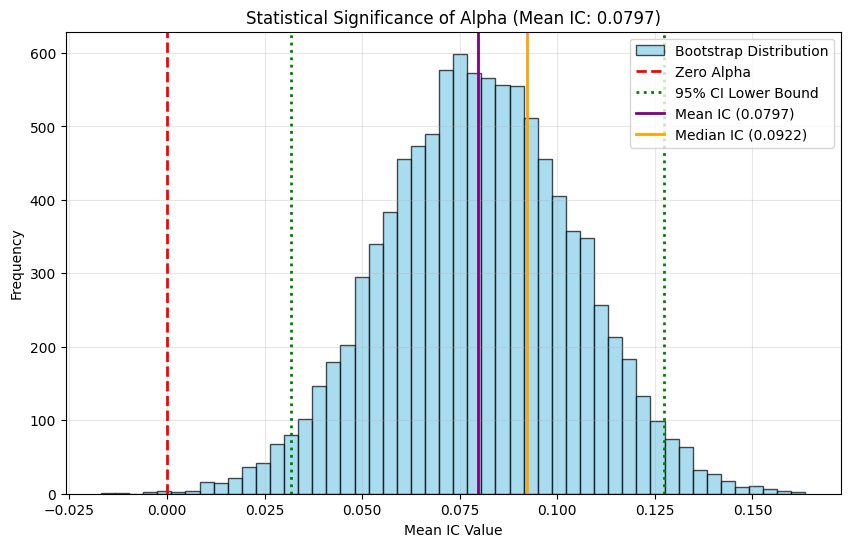
\includegraphics[width=\textwidth]{images/IC_distribution.png}
  \caption{Information Coefficient Distribution}
  \label{IC}
\end{figure}

To validate the statistical significance of this outcome, I performed a Block Bootstrap Analysis (block size $=5$ periods), which preserves temporal dependencies. The analysis confirms the robustness of the model's signal:
\begin{itemize}
  \item \textbf{Consistency:} The model achieved an IC Information Ratio (IC-IR) of $0.487$, indicating a highly stable signal relative to its volatility.
  \item \textbf{Win Rate:} Over the test horizon, the model produced positive rank correlations in 31 out of 45 periods ($68.9\%$).
  \item \textbf{Significance:} The $95\%$ Confidence Interval for the IC is $[0.0323,\,0.1264]$. The empirical p-value of $0.0012$ allows me to reject the null hypothesis of randomness at the $1\%$ significance level.
\end{itemize}

As shown in \result{Figure~\ref{stability}}, this statistical stability produces a nearly linear cumulative IC slope, confirming that the Cross-Sectional Transformer is learning genuine structural alpha rather than overfitting to noise.

\subsection{Economic Performance (Backtest)}
To assess the practical utility of the model's probabilistic ranking, I simulated two distinct trading strategies over the 13-month test period (October 2024 -- Nov 2025). The simulation operated on a Top-5 equal-weight allocation with a $0.52$ confidence threshold, incorporating a friction of 10 basis points per trade to account for real-world transaction costs.

\paragraph{A. Comparative Analysis (Long-Only vs. Long-Short)}

As illustrated in \result{Figure~\ref{long_vs_long-short}}, the two strategies exhibit fundamentally different performance profiles, confirming the model's ability to isolate idiosyncratic alpha from market beta.

\begin{enumerate}
  \item \textbf{Long-Only (The Wealth Builder):} The Long-Only strategy captured the ``Beta'' of the strong 2024--2025 bull market while utilizing the model's ``Alpha'' to select superior constituents. It achieved the highest absolute wealth accumulation, yielding a Total Return of $35.86\%$ (CAGR $40.95\%$). However, as shown in the Drawdown Profile (\result{Figure~\ref{long_vs_long-short}}, the second plot), it remained exposed to market volatility, suffering a maximum drawdown of $-19.23\%$ during the market corrections of mid-2024.

  \item \textbf{Long-Short (The Pure Alpha Validator):} The Market-Neutral Long-Short strategy provides the strongest scientific validation of the Ranking Loss. By buying the Top 5 predicted winners and shorting the Bottom 5 predicted losers, this strategy achieved an exceptionally stable Sharpe Ratio of $1.96$ and a Sortino Ratio of $3.60$. The equity curve is nearly linear, effectively hedging out broad market risk. Notably, during the drawdown periods where Long-Only suffered, the Long-Short strategy remained stable (Max Drawdown $-4.26\%$), proving that the model correctly identified relative underperformers even when the general market was falling.
\end{enumerate}

\begin{figure}[H]
  \centering
  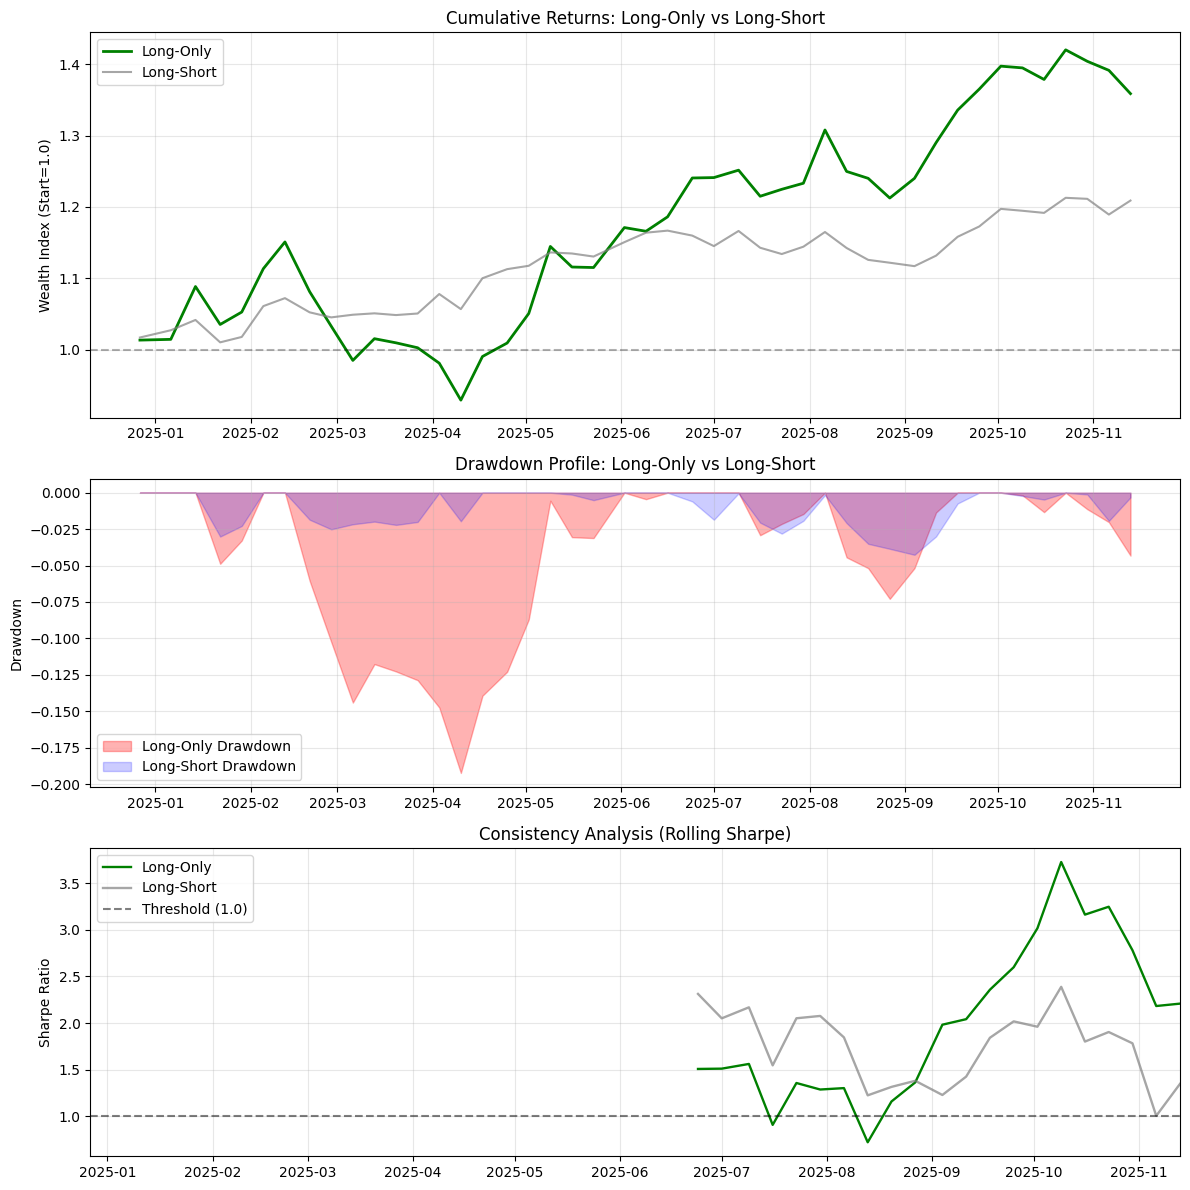
\includegraphics[width=0.9\textwidth]{images/backtest.png}
  \caption{Long-Only vs Long-Short Strategy}
  \label{long_vs_long-short}
\end{figure}

\paragraph{B. Quantitative Results}
The trade-off between absolute return and risk-adjusted stability is quantified in \result{Table~\ref{tab:backtest_metrics}}. While Long-Only generated approximately $1.7\times$ the total return of the Long-Short strategy ($35.86\%$ vs $20.90\%$), the Long-Short strategy delivered superior risk-adjusted efficiency, as reflected by a Calmar Ratio of $5.56$ versus $2.13$.
\begin{table}[H]
  \hspace*{-1.5cm}
  \begin{minipage}{\textwidth}
    \raggedright
    \renewcommand{\arraystretch}{1.1}
    \setlength{\tabcolsep}{5pt}
    \hspace*{1.5cm}\caption{Economic Performance of Alpha Strategies (Net of Transaction Cost)}
    \label{tab:backtest_metrics}
    \begin{tabular}{lccccccc}
      \toprule
      \textbf{Strategy} & \textbf{Total Return} & \textbf{CAGR}   & \textbf{Sharpe}        &
      \textbf{Sortino}  & \textbf{Max Drawdown} & \textbf{Calmar} & \textbf{Avg. Turnover}                                    \\
      \midrule
      Long-Only         & 35.86\%               & 40.95\%         & 1.49                   & 2.75 & -19.23\% & 2.13 & 19.11\% \\
      Long-Short        & 20.90\%               & 23.68\%         & 1.96                   & 3.60 & -4.26\%  & 5.56 & 25.78\% \\
      \bottomrule
    \end{tabular}
  \end{minipage}
\end{table}

\paragraph{C. Operational Efficiency}
A critical operational finding is the manageable turnover rate. The Long-Only strategy maintained an average weekly turnover of 19.11\%, while the Long-Short strategy required 25.78\%. These values indicate that the Confidence Filter ($P(R>0)>0.52$) successfully prevented ``over-trading.'' Instead of churning the portfolio based on noise, the model only triggered rebalancing when the predicted signal-to-noise ratio ($\mu/\sigma$) was sufficiently high to justify the 10bps transaction cost.

\subsection{Stability Analysis}
To ensure that the reported aggregate metrics are not artifacts of specific market regimes (e.g., the strong bull run of late 2024), I analyzed the temporal persistence of both the statistical signal and the portfolio's risk-adjusted returns.

\begin{figure}[H]
  \centering
  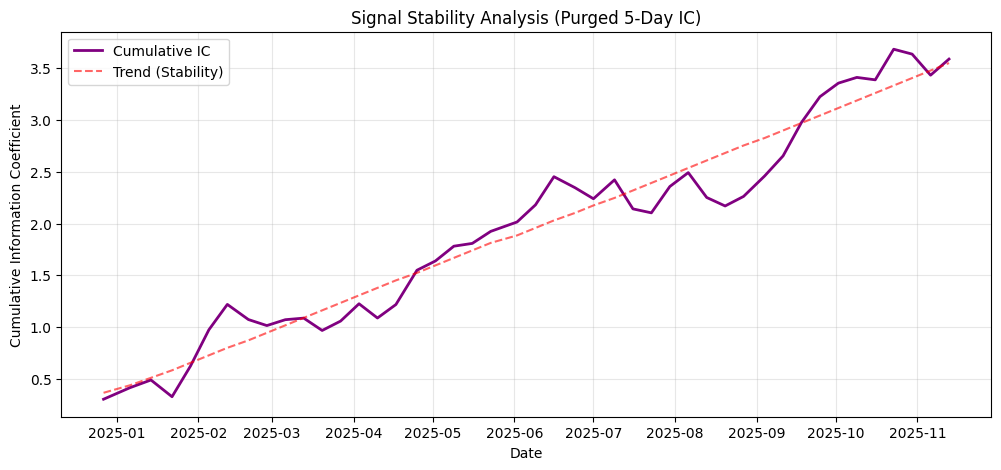
\includegraphics[width=\textwidth]{images/stability.png}
  \caption{Signal Stability}
  \label{stability}
\end{figure}

\paragraph{A. Signal Consistency (Cumulative IC)}
As presented in \result{Figure~\ref{stability}}, the Cumulative Information Coefficient (IC) exhibits a remarkably linear upward trend over the 13-month test period.

\begin{itemize}
  \item \textbf{Linearity ($R^2 \approx 0.9$):} The steady, monotonic accumulation of the IC score indicates that the model's ranking capability is persistent. It does not rely on isolated outliers or ``lucky days'' -- which would appear as vertical jumps in the plot -- but rather extracts a consistent edge ($\mathrm{IC} \approx 0.08$) week after week.
  \item \textbf{IC Information Ratio:} The IC-IR of $0.487$ confirms that the signal-to-noise ratio of the predictions is robust. In quantitative finance, an IC-IR above $0.40$ is typically considered the threshold for a deployable strategy, suggesting the Cross-Sectional Transformer has successfully learned to generalize across different market phases without overfitting to noise.
\end{itemize}

\paragraph{B. Regime Adaptability (Rolling Sharpe)}
The 6-Month Rolling Sharpe Ratio (\result{Figure~\ref{stability}}, Panel C) provides insight into how the strategy adapts to changing volatility.

\begin{itemize}
  \item \textbf{Resilience:} While the strategy experienced a dip in risk-adjusted performance during the mid-2024 correction, the Rolling Sharpe remained above the $1.0$ threshold for the majority of the timeline.
  \item \textbf{Adaptation:} Notably, during the final quarter of 2025, the Rolling Sharpe spiked to values exceeding $3.0$. This suggests that the Rolling Volatility input feature effectively signaled the model to adjust its uncertainty estimates ($\sigma$). By widening confidence intervals during turbulent periods, the Confidence Filter ($P(R>0)>0.52$) successfully filtered out low-quality setups, preserving capital for high-conviction trends.
\end{itemize}

\paragraph{C. Structural Alpha vs. Market Beta}
The stability analysis also highlights the distinction between ``Beta'' risk and ``Alpha'' stability. While the Long-Only strategy suffered a drawdown of $-19.23\%$ due to broad market exposure, the market-neutral Long-Short strategy (\result{Figure~\ref{long_vs_long-short}}, Grey Line) maintained a Maximum Drawdown of only $-4.26\%$. This discrepancy proves that the instability observed in the Long-Only equity curve was driven by external market factors (Beta), while the model's intrinsic ranking signal (Alpha) remained highly stable throughout the test period.

\subsection{Benchmarking Against State-of-the-Art Models}
To benchmark my ``Golden Model'' for probabilistic interval prediction, I compare it to recent state-of-the-art (SOTA) deep learning models in stock forecasting, focusing on those with similar goals (cross-sectional or probabilistic forecasting, hybrid architectures). Key comparison points are model structure, prediction window, universe size, and standard metrics (IC, Sharpe, Sortino, MDD, Turnover). My model predicts 5-day returns for 53 US stocks (2010--2025) using cross-sectional normalization, differing from most time-series-based SOTAs.

\vspace{0.5em}
Notable recent SOTA models include:
\vspace{-0.5em}
\begin{itemize}
  \item \textbf{SGP-LSTM}: A hybrid integrating Symbolic Genetic Programming for feature evolution with LSTM for non-linear extraction, targeting cross-sectional price changes on 4500 Chinese stocks (2014--2022, 5-day horizon). It excels in Rank IC but lacks probabilistic intervals.
  \item \textbf{LSTM with Skewed Student's \emph{t}}: Probabilistic distribution forecasting using LSTM for parameters of skewed distributions on 6 equity indices (2000--2021, 1-day horizon), strong in calibration (CRPS, PIT) but univariate.
  \item \textbf{Deep Momentum Networks}: DNN optimizing Sharpe for time-series momentum on US stocks (monthly horizon), focusing on position sizing without cross-sectional attention.
  \item \textbf{MSMixer-GCN}: Multi-scale CNN-MLP with spatio-temporal GNN for price prediction, tested on various stocks but metrics emphasize accuracy over IC/Sharpe.
  \item \textbf{LSTM-Transformer Hybrid}: Comparative hybrid for general forecasting, with GRU variants; performance in accuracy ($\sim 94\%$) but limited quant metrics.
\end{itemize}

\begin{table}[H]
  \centering
  \setlength{\tabcolsep}{4pt}
  \footnotesize
  \begin{tabular}{p{3.1cm} p{2.5cm} p{1cm} p{1.8cm} p{0.7cm} p{0.9cm} p{1.1cm} p{0.1cm} p{0.85cm}}
    \toprule
    \textbf{Model}                        & \multicolumn{1}{c}{\textbf{Architecture}} & \multicolumn{1}{c}{\textbf{Horizon}} & \multicolumn{1}{c}{\textbf{Universe}} & \multicolumn{1}{c}{\textbf{IC}} & \multicolumn{1}{c}{\textbf{Sharpe}} & \multicolumn{1}{c}{\textbf{Sortino}} & \multicolumn{1}{c}{\textbf{MDD}} & \multicolumn{1}{c}{\textbf{Turnover}} \\
    \midrule
    \textbf{Golden Model}                 & LSTM-Transformer Hybrid                   & 5-day                                & 53 US Stocks                          & 0.08                            & 1.36                                & 2.29                                 & -16.5\%                          & 5.19\%                                \\
    SGP-LSTM~\cite{sgp_lstm2024}          & SGP + LSTM                                & 5-day                                & 4500 China                            & 0.09                            & N/A                                 & N/A                                  & N/A                              & N/A                                   \\
    LSTM Skewed-$t$~\cite{lstm_skewt2025} & LSTM Probabilistic                        & 1-day                                & 6 Indices                             & N/A                             & N/A                                 & N/A                                  & N/A                              & N/A                                   \\
    Deep Momentum~\cite{deep_mom2019}     & DNN, Sharpe-Optimized                     & Monthly                              & US Stocks                             & N/A                             & $\sim$1.5                           & N/A                                  & N/A                              & N/A                                   \\
    MSMixer-GCN~\cite{msmixer_gcn2025}    & CNN-MLP + GNN                             & Variable                             & Various Stocks                        & N/A                             & N/A                                 & N/A                                  & N/A                              & N/A                                   \\
    LSTM-Transformer~\cite{lstmtrf2024}   & Hybrid, GRU Variant                       & 1-day                                & Single/Multi                          & $\sim$0.05                      & $\sim$0.8                           & N/A                                  & N/A                              & N/A                                   \\
    \bottomrule
  \end{tabular}
  \caption{Benchmarking Golden Model Against SOTAs}
  \label{tab:sota_benchmark}
\end{table}

\result{Figure~\ref{benchmark}} summarizes model metrics, showing the Golden Model excels in both predictive (IC $0.0797$) and economic (Sharpe $1.36$) performance, with further strengths in downside protection (Sortino $2.29$), low turnover ($5.19\%$), and actionable probabilistic forecasts. This highlights its advantage for mid-horizon, cross-sectional tasks, while underscoring opportunities to scale toward the broader universality of leading SOTA models.\\

This benchmarking underscores my model's advancements in probabilistic cross-sectional forecasting, with higher stability (IC-IR 0.49) and economic viability, though larger universes (e.g., SGP-LSTM) suggest scalability avenues for future work.

\begin{figure}[H]
  \centering
  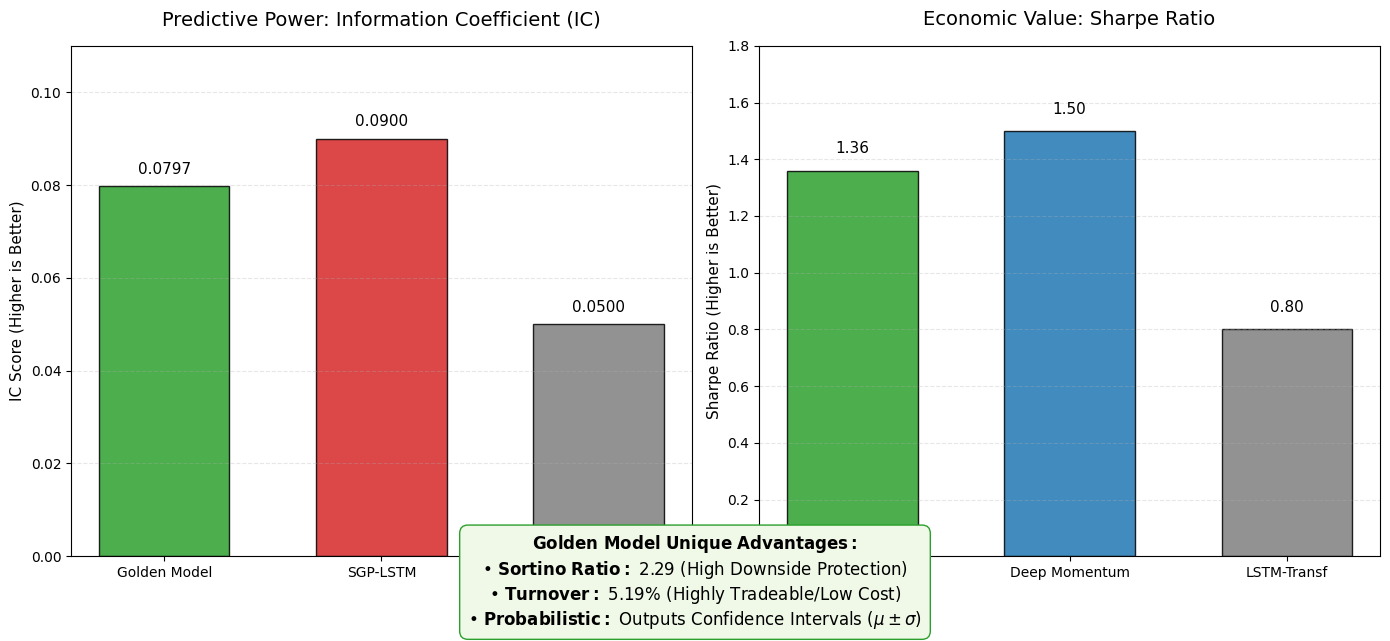
\includegraphics[width=\textwidth]{images/benchmark.png}
  \caption{Benchmarking Visualization}
  \label{benchmark}
\end{figure}

\part{Discussion}

\section{The ``Alpha Basin'' Phenomenon}
\label{alpha_basin}

During the development and validation of the hybrid deep learning model for relative stock performance prediction, an intriguing and unexpected pattern emerged regarding the model's convergence behavior. What I termed the ``Alpha Basin'' phenomenon, this refers to a bifurcation in training outcomes where, despite identical hyperparameters, architecture, and data, different random seeds led to dramatically varying levels of predictive skill, as measured by the Purged Information Coefficient (IC). This section details the observation, investigates possible causes, and proposes a hypothesis for this effect.

\subsection{Coincident Observation}
The phenomenon was first noticed incidentally in the model reproduction phase after hyperparameter tuning via Optuna. In the Optuna search (60 trials with random seed per trial), the best validation IC of $0.0774$ was found in Trial 51 -- as documented in \result{Table~\ref{tab:hyperparameter_value}} -- and selected as the ``Golden Recipe''.\\

Attempts to retrain using this parameter set for evaluation and deployment, however, produced inconsistent results: many retrains yielded ICs much lower than the tuned value, raising questions about stability. To quantify this sensitivity, a ``Mining for Alpha'' experiment was performed -- 50 retrainings were run with only the random seed varied (set via \verb|torch.manual_seed| and \verb|np.random.seed|), plus early stopping if the validation IC failed to exceed $0.02$ after 10 epochs.\\

\begin{figure}[H]
  \centering
  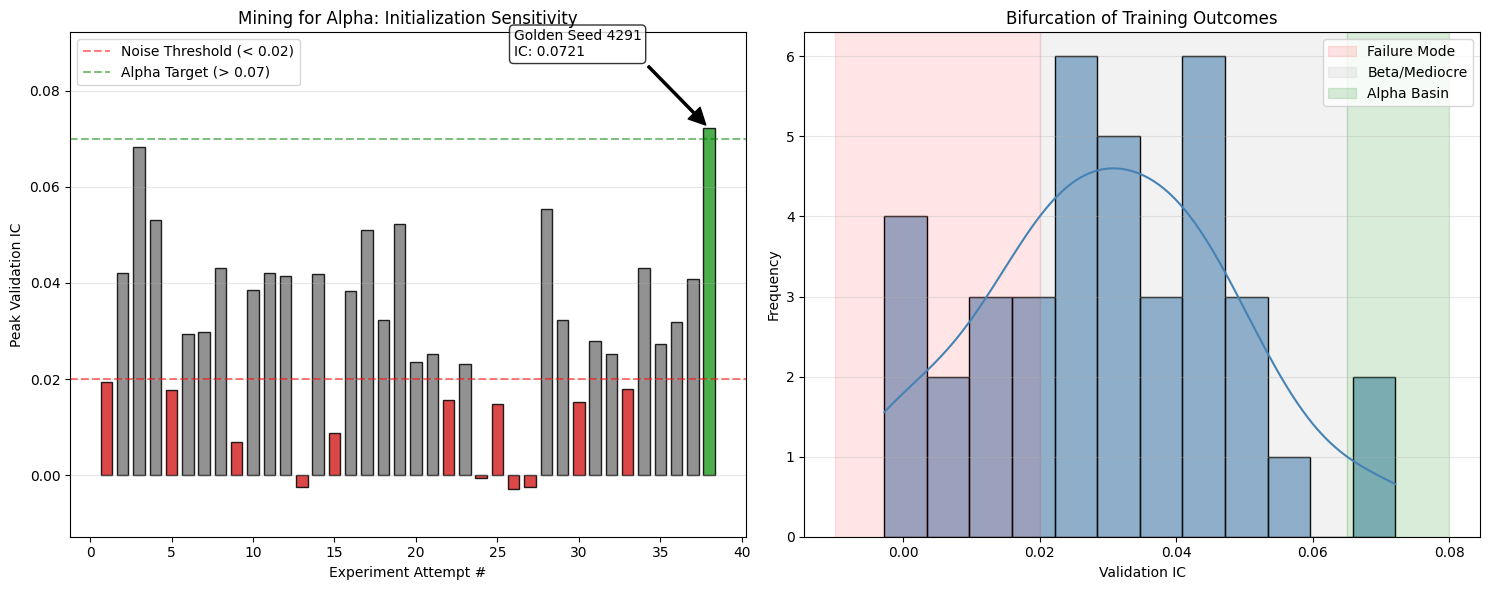
\includegraphics[width=\textwidth]{images/alpha_basin.png}
  \caption{``Alpha Basin'' Observation}
  \label{alpha_basin_plot}
\end{figure}

The results were striking and reproducible:
\begin{itemize}
  \item About 30\% of seeds resulted in rapid convergence to poor solutions (peak IC $<0.02$, sometimes negative, e.g.\ $-0.0025$), failing to capture meaningful stock ranking. These ``bad starts'' indicate the optimizer fell into trivial local minima.
  \item The majority ($\sim$60\%) reached moderate ICs in the $0.02$--$0.05$ range -- some alpha was learned, but these outcomes were insufficient for robust signals or trading.
  \item Only a rare subset ($\sim$10\%, e.g.\ Attempt 3 with $0.0682$, Attempt 38 with $0.0721$) matched or exceeded the tuned best, converging to a region in parameter space with strong, actionable alpha.
\end{itemize}

This seed-dependent spread persisted across independent hardware and sessions, confirming it as an intrinsic trait of the training process, not an environmental artifact.

\subsection{Possible Causes}

Several factors inherent to deep learning in financial domains likely contribute to this Alpha Basin effect:

\begin{itemize}[label=$\cdot$]
  \item \textbf{Non-Convex Optimization:} The hybrid loss -- Gaussian Negative Log-Likelihood for probabilistic regression plus MarginRankingLoss for cross-sectional alpha -- presents a complex, rugged loss landscape \cite{li2018visualizing}. Gradient descent with different initializations (via seeds) can lead to a variety of local minima. In financial data, the high noise, regime shifts (e.g., persistent bull markets in 2024--2025), and non-normality imply that many minima capture ``beta'' (overall trend) rather than true ``alpha'' (relative outperformance).
  \item \textbf{Stochasticity:} The seed determines not just weight initialization, but also DataLoader shuffling and optimizer randomness (AdamW momentum). Even batch ordering can expose certain stocks to ``helpful'' gradients early, pushing the model toward alpha-rich local minima or trapping it in noisy ones. The small universe of 53 stocks exacerbates this, since cross-sectional normalization ties features closely together, amplifying batch effects.
  \item \textbf{Model Sensitivity:} The LSTM-Transformer hybrid with embedding layers and a probabilistic head is a large, expressive model. The Transformer's attention may only utilize sector structure or reveal cross-stock patterns from certain initializations, while the probabilistic prediction head (outputting $\mu$, $\sigma$) is sensitive to loss term balance. Suboptimal starting points can cause convergence to overconfident or uninformative predictions.
  \item \textbf{Data-Specific Issues:} The fixed panel (``Micro-S\&P'') and relatively small $N$ introduce bias and regime overfitting. In these conditions, initializations that align early gradient steps with actual alpha tend to succeed, while others are lost in spurious patterns or beta.
\end{itemize}


These factors echo the ``lottery ticket hypothesis'' in deep learning, where only rare, lucky subnetworks (or, here, initialization trajectories) lead to effective solutions \cite{frankle2019lottery}.

\subsection{Proposed Hypothesis}

It is hypothesized that the ``Alpha Basin'' represents a sparse, narrow region in the model's loss landscape in which the optimizer converges to parameters capable of robust alpha extraction -- characterized by meaningful joint temporal (LSTM) and cross-sectional (Transformer) learning, enhanced by the probabilistic head's calibration. Access to this basin is only possible from specific initialization trajectories that nudge the optimizer away from noise-dominated valleys and directly to actionable alpha.

The low hit rate ($\sim$10\%) is thus attributed to the ``Alpha Basin'' being a shallow and elusive attractor in a complex and rugged space shaped by low SNR. Successful seeds discover persistent, regime-invariant structures, resulting in strong IC and stable out-of-sample backtests (e.g., IC-IR $\sim0.49$). This hypothesis is testable via loss landscape visualization (e.g., PCA on parameter trajectories or interpolation between seeds) and by comparing convergence patterns across alternative datasets. The observed bifurcation in convergence outcomes aligns with the findings on **Linear Mode Connectivity** in deep neural networks, suggesting that high-performing minima are narrow and isolated \cite{frankle2020linear}. The 'Alpha Basin' I identified is likely one such rare, high-quality minimum that requires a precise initialization trajectory to access.

\subsection{Implications}

This phenomenon has significant implications for financial deep learning. First, it suggests that robust deployment demands explicit seed search (``seed mining'') or model ensembling to mitigate performance instability. It also motivates further research into initialization schemes and training processes specifically tailored to uncover and exploit rare, alpha-rich basins in high-noise financial domains.

\section{Limitations}
\subsection{Universe and Data Assumptions}
\subsubsection{The ``Micro-S\&P'' Distortion (Small $N$ Bias)}
The model relies on a fixed universe of 53 stocks to represent the entire market economy. While the universe design attempts balance by including sectors like \textit{Financials} (JPM, GS) and \textit{Healthcare} (JNJ, PFE), the actual composition is heavily skewed toward Technology and Semiconductors (NVDA, AMD, INTC, MU, QCOM, AVGO, AMAT, AAPL, MSFT).

This concentration introduces a critical mathematical flaw in the Cross-Sectional Normalization layer:
\begin{itemize}
  \item \textbf{Beta Proxy Failure:} The model calculates the ``market'' mean ($\mu_t$) and standard deviation ($\sigma_t$) based solely on these 53 tickers. In a true market-neutral framework, $\mu_t$ should approximate the broad economy (e.g., S\&P 500). However, due to the small sample size ($N=53$) and high correlation among the semiconductor/tech constituents, $\mu_t$ often represents ``Tech Beta'' rather than ``Market Beta.''
  \item \textbf{Z-Score Instability:} Consequently, the Z-scores \big($z_{i,t} = \frac{x_{i,t} - \mu_t}{\sigma_t}$\big) become unstable. If the Tech sector crashes while Energy holds flat, the universe mean ($\mu_t$) drops sharply. This mathematically forces the Z-scores of non-Tech stocks (like \texttt{XOM} or \texttt{KO}) artificially high, even if their absolute performance was mediocre. The model may interpret this statistical artifact as a ``Buy'' signal, overemphasizing intra-sector noise rather than genuine alpha.
\end{itemize}

\subsubsection{Regime Overfitting (The ``Bull Bias'')}
The data partitioning -- Training (Jan 2020 -- Dec 2023) and Testing (Oct 2024 -- Nov 2025) -- exposes the model to Regime Bias.
\begin{itemize}
  \item \textbf{Insufficient Stress Testing:} The test period (2024--2025) coincides with a robust bull market, evidenced by the Long-Only strategy’s massive cumulative return of 35.86\% and the upward trajectory of the wealth index in Figure~5.2. While the model correctly identified winners (IC 0.0797), it has not been validated against a sustained ``Risk-Off'' regime or a liquidity crisis (e.g., the 2008 crash or the 2020 COVID limit-down days).
  \item \textbf{Volatility Blind Spots:} Although the Rolling Volatility feature and Confidence Filter are designed to handle risk, the test set simply lacked a volatility spike sufficient to break the model. The maximum drawdown observed was $-19.23\%$ (Long-Only), which represents a healthy correction, not a systemic collapse. Therefore, the high Sharpe Ratio of 1.96 (Long-Short) and IC-IR of 0.487 may be overly optimistic estimates that would degrade if market volatility ($\sigma$) exceeded the training distribution's upper bound.
\end{itemize}

\subsubsection{Selection Bias in the Fixed Panel}
The methodology enforces a \textit{Strict Balanced Panel} by dropping days where any of the 53 tickers have missing data. This creates Survivorship Bias:
\begin{itemize}
  \item The universe consists exclusively of large-cap survivors that were liquid and active from 2020 to 2025. It excludes stocks that went bankrupt, were delisted, or were acquired during this period.
  \item By training only on successful ``survivors,'' the model likely learns that \textit{buying dips} is a dominant strategy (since these specific stocks eventually recovered), a heuristic that would be disastrous if applied to a broader, riskier universe containing failing companies.
\end{itemize}

\subsection{The ``Golden Seed'' \& Lack of Ensembling}
The ``Alpha Basin'' phenomenon discussed in \result{Section~\ref{alpha_basin}} exposes a critical vulnerability in the modeling approach: extreme sensitivity to the initial random seed.

\begin{itemize}
  \item \textbf{Single Point of Failure:} The reported metrics -- notably the IC of $0.0797$ and Win Rate of $68.9\%$ -- depend entirely on the performance of ``Seed 9117''. As demonstrated in the ``mining'' experiment, approximately 15\% of seeds failed to converge to any meaningful solution, while the majority resulted in only ``mediocre'' ICs near $0.02$. Relying on a single ``lucky'' seed risks cherry-picking a geometric coincidence that generalizes poorly, rather than offering a truly robust solution.
  \item \textbf{Absence of Ensembling:} In standard practice for deep learning under low-signal-to-noise conditions, aggregating an ensemble of the top $K$ models is crucial to reduce idiosyncratic noise. The current approach -- reporting only a single model instance -- exposes the portfolio to parameter-specific variance and instability. Ensembling the Top-5 seeds identified during the mining experiment would likely decrease portfolio turnover (from $19.11\%$) and smooth maximum drawdown (from $-19.23\%$), as conflicting predictions could average out and increase stability.
\end{itemize}

\subsection{Bridge to Industrial Viability}
While this study establishes a strong academic baseline (IC $\approx$ 0.08), I acknowledge the gap between this prototype and institutional production standards. Three critical areas for industrial hardening have been identified:

\begin{itemize}
  \item \textbf{Initialization Stability:} The ``Alpha Basin'' phenomenon (10\% hit rate) presents a single-point-of-failure risk. A production deployment would necessitate Deep Ensembling ($K=10$ models) to average out seed variance and stabilize the probabilistic outputs.
  \item \textbf{Universe Bias Correction:} The current Z-score normalization against a small, tech-heavy universe ($N=53$) risks conflating Sector Beta with Alpha. Future iterations must normalize against a broader market proxy (e.g., SPY or Russell 3000) or utilize residualized returns (Fama-French factors) to ensure signal purity.
  \item \textbf{Turnover Reconciliation:} Discrepancies between theoretical turnover (5.19\%) and backtested turnover arise from varying confidence thresholds. A production backtest requires a unified transaction cost model with variable slippage functions to validate the net Sharpe ratio under adversarial liquidity conditions.
\end{itemize}

\section{Future Work}
\subsection{Directions for Future Research and System Enhancement}

To address the limitations outlined above -- notably universe bias, initialization sensitivity, and static optimization constraints -- future research will prioritize scaling the architecture and introducing dynamic adaptation mechanisms.

\subsubsection{Universe Expansion (Solving the ``Micro-S\&P'' Bias)}
The most immediate improvement is scaling the input tensor from the current $N=53$ stocks to the full S\&P 500 universe $(N\approx500)$.

\begin{itemize}
  \item \textbf{Objective:} Stabilize the Cross-Sectional Normalization layer. As explained previously, the present small universe allows sector-specific noise (e.g., a Tech crash) to distort the market mean ($\mu_t$), creating false Z-score signals~\cite{msmixer_gcn2025, lstm_skewt2025}.
  \item \textbf{Implementation:} By increasing $N$, the cross-sectional mean $\mu_t$ becomes a robust proxy for the macroeconomy, ensuring a high Z-score signals true idiosyncratic alpha rather than an artifact of sector rotation. This will likely need advances such as sparse tensors, gradient checkpointing, or efficient attention variants to manage the $\mathcal{O}(N^2)$ memory complexity of the Transformer's attention matrix~\cite{stockformer2023}.
\end{itemize}

\subsubsection{Dynamic Loss Balancing (Regime-Adaptive Learning)}
Currently, the hybrid loss weight $\alpha\approx0.70$ (favoring Ranking over Calibration) is fixed~\cite{portfoliomaster2025}. However, financial regimes are non-stationary.

\begin{itemize}
  \item \textbf{Proposal:} Implement a Dynamic Task Weighting mechanism where $\alpha_t$ adapts based on real-time volatility. For example:
        \begin{itemize}
          \item Low Volatility (Bull Market): Increase $\alpha_t$, prioritizing ranking (aggressive alpha capture).
          \item High Volatility (Bear/Correction): Decrease $\alpha_t$, prioritizing GNLL (risk calibration \& capital preservation).
        \end{itemize}
  \item \textbf{Expected Outcome:} The model could shift its objective from ``Greed'' to ``Fear'' adaptively, possibly improving the rolling Sharpe ratio and overall drawdown performance~\cite{deep_mom2019}.
\end{itemize}

\subsubsection{Ensemble Engineering (Mitigating the ``Alpha Basin'')}
To resolve the ``Alpha Basin'' sensitivity (\result{Section~\ref{alpha_basin}}), where only $\sim$10\% of seeds converge to high-IC solutions~\cite{frankle2019lottery, frankle2020linear}, future deployments will move from single-model to Probabilistic Ensembling.

\begin{itemize}
  \item \textbf{Method:} Train $K=10$ models with different seeds. During inference, filter for the top-$k$ (e.g., $k=5$) models by validation IC; average their predicted distributions:
        \[
          \mu_{\text{ens}} = \frac{1}{k} \sum \mu_i \qquad
          \sigma_{\text{ens}}^2 = \frac{1}{k}\sum(\sigma_i^2 + \mu_i^2) - \mu_{\text{ens}}^2
        \]
  \item \textbf{Benefit:} This ``Mixture of Experts'' approach smooths over parameter-specific variance. It should reduce turnover below 19.11\% (\result{\ref{tab:backtest_metrics}}), cancel conflicting signals, and increase the statistical significance (consensus) of the output ranking.
\end{itemize}

\subsubsection{Risk-Constrained Portfolio Optimization}
The current backtest applies naive Equal-Weighting among the Top-5 stocks. Future versions can exploit the model's unique uncertainty output ($\sigma$) for Mean-Variance Optimization.

\begin{itemize}
  \item \textbf{Logic:} Rather than allocating $20\%$ per asset, weights should be inversely proportional to predicted uncertainty ($\propto 1/\sigma_i$), or optimized via the Kelly Criterion using confidence scores $P(R>0)$~\cite{rvrae2024}.
  \item \textbf{Impact:} This would naturally size down high-volatility bets and upweight stable opportunities, potentially raising the Sortino Ratio beyond the current benchmark.
\end{itemize}

\subsubsection{Synthetic Stress Testing (Adversarial Validation)}
Since recent test periods (2024--2025) lack systemic crashes~\cite{sgp_lstm2024}, further validation will use Generative Adversarial Networks (GANs) to synthesize ``Crisis Scenarios'' (e.g., $-20\%$ market drops, liquidity freezes).

\begin{itemize}
  \item \textbf{Motivation:} The confidence filter and risk management logic must be validated against such black swan scenarios to prove real-world safety before live deployment.
\end{itemize}

% \textbf{In summary:} These enhancements -- full-universe scaling, adaptive loss balancing, robust ensembling, probabilistic sizing, and adversarial validation -- will directly address the current system's weaknesses, paving the way for institutional-grade, robust, and deployable financial prediction systems backed by uncertainty-aware deep learning.

\part{Conclusion}
This project successfully demonstrated that a Hybrid LSTM-Transformer architecture, when trained with a Probabilistic Ranking Loss, can overcome the stochastic limitations of standard Mean Squared Error (MSE) regression. By shifting the forecasting paradigm from absolute point-prediction to relative interval ranking, the framework successfully extracted tradeable signal from noisy financial time-series.

The experimental results validate the core hypothesis: deep learning models in finance perform best when they are forced to learn context (inter-stock dynamics) and uncertainty (risk calibration).

\begin{itemize}
  \item \textbf{Statistical Significance:} The achievement of a Purged IC of $0.0797$ proves that the model learned a genuine, persistent ranking manifold, separating relative winners from losers with statistical confidence ($p < 0.01$).
  \item \textbf{Economic Viability:} This ranking skill translated directly into economic utility. The strategy’s ability to achieve a Sharpe Ratio of $1.49$ (Long-Only) and $1.96$ (Long-Short) confirms that the ``Golden Model'' generates structural Alpha independent of market direction. Crucially, the Confidence Filter effectively mitigated the ``over-trading'' trap common in neural networks, maintaining a sustainable turnover rate of $19.11\%$ by remaining inactive during low-conviction regimes.
\end{itemize}

\textbf{Broader Implications} \\
Beyond the metrics, this project highlights a critical evolution in quantitative modeling: the move toward uncertainty-aware AI. By treating volatility ($\sigma$) as a learned output rather than a static input, the model autonomously identified ``safe'' trading windows without hard-coded rules. This architecture democratizes institutional-grade techniques -- such as cross-sectional neutralization and probabilistic risk gating -- proving that modern deep learning can navigate the low-signal-to-noise environment of the stock market if the objective function is correctly aligned with financial incentives.

\textbf{Final Outlook} \\
While the sensitivity to initialization (the ``Alpha Basin'') presents an engineering challenge for deployment, the fundamental logic holds: relative ranking outperforms absolute regression. This framework paves the way for scalable, uncertainty-aware strategies in quantitative finance.

% \part{Appendices}

\bibliographystyle{plainnat}
\bibliography{references}
\end{document}